% ===============================================================
%  Relatório Final — ENGCIA (Engenharia do Conhecimento)
%  Sistema Pericial de Apoio à Decisão em Veículos Autónomos
%
%  Compilar (nesta pasta), com XeLaTeX ou Tectonic:
%      tectonic relatorio.tex
%  ou  xelatex relatorio.tex   (duas vezes, para o índice e as referências)
% ===============================================================

\documentclass[11pt,a4paper,oneside]{report}

% ---------------------------------------------------------------
% metadados.tex — dados da capa e das propriedades do PDF.
% Para alterar a capa, basta editar este ficheiro.
% ---------------------------------------------------------------

\newcommand{\instituicao}{Instituto Superior de Engenharia do Porto}
\newcommand{\curso}{Mestrado em Engenharia de Inteligência Artificial}
\newcommand{\uc}{Engenharia do Conhecimento}
\newcommand{\ucsigla}{ENGCIA}
\newcommand{\anoletivo}{2026/2027}
\newcommand{\semestre}{1.º Semestre}

\newcommand{\tituloprincipal}{Sistema Pericial de Apoio à Decisão em Veículos Autónomos}
\newcommand{\subtitulo}{Relatório Final}
\newcommand{\descricao}{Aquisição, representação e implementação:\\
conhecimento pericial em \emph{Drools}}

\newcommand{\datarelatorio}{25 de outubro de 2026}

% Autores: uma linha \autor{nome}{email} por elemento (a capa adapta-se).
\providecommand{\autor}[2]{}
\newcommand{\listaautores}{%
  \autor{Ana Salomé Ferreira Teixeira}{1210803@isep.ipp.pt}%
  \autor{Diogo Miguel Gonçalves Ribeiro}{1260429@isep.ipp.pt}%
  \autor{João Gabriel Domingos de Azevedo}{1211519@isep.ipp.pt}%
  \autor{Pedro Nuno Verde Cerqueira}{1260443@isep.ipp.pt}%
  \autor{Rúben Alexandre Abreu Freitas}{1231267@isep.ipp.pt}%
  \autor{Rúben Carlos Zamith Ribeiro}{1161532@isep.ipp.pt}%
}
\newcommand{\autoresmeta}{Ana Salomé Ferreira Teixeira, Diogo Miguel Gonçalves Ribeiro,
  João Gabriel Domingos de Azevedo, Pedro Nuno Verde Cerqueira, Rúben Alexandre Abreu Freitas,
  Rúben Carlos Zamith Ribeiro}

% Docentes: uma linha \docente{nome} por elemento.
\providecommand{\docente}[1]{}
\newcommand{\listadocentes}{%
  \docente{Luiz Felipe Rocha de Faria}%
  \docente{Vítor Rafael Palmeiro Crista}%
  \docente{Diogo Ferreira Risca}%
}

% ---------------------------------------------------------------
% preambulo.tex — pacotes, tipos de letra, cores e estilos
% Tipos de letra iguais aos do Word: Book Antiqua (texto),
% Georgia (títulos) e Aptos (legendas). Requer XeLaTeX/Tectonic.
% ---------------------------------------------------------------

\usepackage{fontspec}
\usepackage[portuguese]{babel}
\usepackage{microtype}

\setmainfont{Book Antiqua}[AutoFakeBold=1.5,AutoFakeSlant=0.2]
\setmonofont{Consolas}[Scale=0.9]
\newfontfamily\titulos{Georgia}
\newfontfamily\legendas{Aptos}[Path=fontes/,Extension=.ttf,
  UprightFont=*-Regular,BoldFont=*-Bold,ItalicFont=*-Italic,BoldItalicFont=*-BoldItalic]
% Símbolos que a Book Antiqua não tem (setas, etc.)
\newfontfamily\simbolosB{Cambria}
\newfontfamily\simbolos{Segoe UI Symbol}

\usepackage[a4paper,margin=2.5cm]{geometry}
\usepackage{graphicx}
\usepackage{array}
\usepackage{longtable}
\usepackage[table]{xcolor}
\usepackage{float}
\usepackage{pdflscape}
\usepackage{enumitem}
\usepackage{caption}
\usepackage{titlesec}
\usepackage[titles]{tocloft}
\usepackage{fancyhdr}
\usepackage{csquotes}
\usepackage{url}
\usepackage[most]{tcolorbox}
\usetikzlibrary{positioning,arrows.meta,calc,fit}

% --- Cores -----------------------------------------------------
\definecolor{corEscura}{HTML}{1F3A5F}
\definecolor{corDestaque}{HTML}{AD451D}
\definecolor{corCinza}{HTML}{5A6672}
\definecolor{corFundo}{HTML}{F4F6F8}
\definecolor{corLegenda}{HTML}{404040}

% --- Parágrafos: texto justificado, sem avanço, espaço entre parágrafos
\setlength{\parindent}{0pt}
\setlength{\parskip}{6pt plus 2pt}
\linespread{1.08}
\setlength{\emergencystretch}{2em}
\setlist{itemsep=2pt,parsep=0pt,topsep=4pt}

% --- Títulos (Georgia) -----------------------------------------
\titleformat{\chapter}[hang]
  {\titulos\fontsize{20}{24}\selectfont\bfseries\color{corEscura}}{\thechapter.}{0.5em}{}
\titleformat{name=\chapter,numberless}[hang]
  {\titulos\fontsize{20}{24}\selectfont\bfseries\color{corEscura}}{}{0pt}{}
\titlespacing*{\chapter}{0pt}{0pt}{18pt}
\titleformat{\section}
  {\titulos\fontsize{12.5}{15}\selectfont\bfseries\color{corEscura}}{\thesection.}{0.5em}{}
\titlespacing*{\section}{0pt}{16pt}{6pt}
\titleformat{\subsection}
  {\titulos\fontsize{11.5}{14}\selectfont\bfseries\itshape\color{corEscura}}{\thesubsection.}{0.5em}{}

% Anexo: \anexo{A}{Título} — título sem número de capítulo, entrada no índice.
\newcommand{\anexo}[2]{\chapter*{Anexo #1 – #2}\addcontentsline{toc}{chapter}{Anexo #1 – #2}}

% --- Legendas (Aptos, centradas) -------------------------------
\DeclareCaptionFont{legenda}{\legendas\fontsize{9}{11}\selectfont\color{corLegenda}}
\captionsetup{font=legenda,labelsep=endash,justification=centering,singlelinecheck=false,skip=6pt}
\captionsetup[table]{position=top}

% Figuras e tabelas numeradas de forma seguida (como no Word).
\counterwithout{figure}{chapter}
\counterwithout{table}{chapter}

% --- Índice e listas (como no Word) ----------------------------
\addto\captionsportuguese{%
  \renewcommand{\contentsname}{Índice}%
  \renewcommand{\listfigurename}{Lista de figuras}%
  \renewcommand{\listtablename}{Lista de tabelas}%
  \renewcommand{\bibname}{Bibliografia}%
}
\renewcommand{\cfttoctitlefont}{\titulos\fontsize{20}{24}\selectfont\bfseries\color{corEscura}}
\renewcommand{\cftloftitlefont}{\cfttoctitlefont}
\renewcommand{\cftlottitlefont}{\cfttoctitlefont}
\renewcommand{\cftchapdotsep}{\cftdotsep}
\renewcommand{\cftfigpresnum}{Figura }
\renewcommand{\cftfigaftersnum}{ –}
\setlength{\cftfignumwidth}{5.6em}
\renewcommand{\cfttabpresnum}{Tabela }
\renewcommand{\cfttabaftersnum}{ –}
\setlength{\cfttabnumwidth}{5.6em}
\setlength{\cftfigindent}{0pt}
\setlength{\cfttabindent}{0pt}
% Sem espaço entre capítulos nas listas de figuras e de tabelas (como no Word).
\usepackage{etoolbox}
\makeatletter
\patchcmd{\@chapter}{\addtocontents{lof}{\protect\addvspace{10\p@}}}{}{}{}
\patchcmd{\@chapter}{\addtocontents{lot}{\protect\addvspace{10\p@}}}{}{}{}
\makeatother
\urlstyle{same}

% --- Número de página centrado no rodapé -----------------------
\pagestyle{plain}

% --- Tabelas (estilo do Word: cabeçalho azul, linhas alternadas)
\newcolumntype{L}[1]{>{\raggedright\arraybackslash}p{#1}}
\newcommand{\cab}[1]{{\color{white}\bfseries #1}}
\newcommand{\linhacab}{\rowcolor{corEscura}}
% \begin{tabela}{colunas} ... \end{tabela}: longtable em letra pequena, com quebra de página.
\newenvironment{tabela}[1]
  {\par\begingroup\footnotesize\renewcommand{\arraystretch}{1.35}%
   \setlength{\LTpre}{6pt}\setlength{\LTpost}{6pt}%
   \arrayrulecolor{corEscura}\begin{longtable}{#1}}
  {\end{longtable}\endgroup}

% --- Caixas e macros -------------------------------------------
% Estrutura das regras (SE ... ENTÃO ...).
\newtcolorbox{caixaregra}{enhanced, colback=corFundo, colframe=corEscura,
  boxrule=0pt, leftrule=1.2pt, arc=0pt, outer arc=0pt, left=8pt, right=8pt,
  top=4pt, bottom=4pt, fontupper=\ttfamily\small, width=0.75\linewidth, center}
% Versaletes simuladas (a Book Antiqua não as tem), como faz o Word: \pv{texto} escreve
% minúsculas como maiúsculas pequenas (80%). Usado na capa.
\newcommand{\pv}[1]{{\fontsize{0.8\dimexpr\csname f@size\endcsname pt\relax}{0}\selectfont #1}}
% Nomes de componentes e identificadores do código.
\newcommand{\cod}[1]{\texttt{#1}}

\usepackage[hidelinks,bookmarks=true]{hyperref}
\hypersetup{pdftitle={\tituloprincipal},pdfauthor={\autoresmeta},pdflang={pt-PT}}


\begin{document}

% ---------------------------------------------------------------
% capa.tex — página de rosto (dados em metadados.tex)
% ---------------------------------------------------------------
\begin{titlepage}
\centering

\noindent
\begin{minipage}[c]{0.60\textwidth}\raggedright
  
\includegraphics[width=5.2cm]{logos/ISEP_logo.pdf}
\end{minipage}%
\hfill
\begin{minipage}[c]{0.32\textwidth}\raggedleft
  
\includegraphics[trim=92bp 163bp 72bp 160bp,clip,height=2.0cm]{logos/MEIA_logo.jpg}
\end{minipage}

\vspace{0.6cm}
{\fontsize{14}{17}\selectfont\color{corEscura}I\pv{NSTITUTO} S\pv{UPERIOR} \pv{DE} E\pv{NGENHARIA} \pv{DO} P\pv{ORTO}\par}
\vspace{0.25cm}
{\large\color{corCinza}\curso\par}

\vspace{0.4cm}
{\color{corEscura}\rule{\textwidth}{0.9pt}}
\vspace{0.4cm}

{\titulos\large\bfseries\color{corDestaque}\uc{} (\ucsigla)\par}
\vspace{0.15cm}
{\color{corCinza}\anoletivo{} \textperiodcentered{} \semestre\par}

\vspace{0.4cm}
{\color{corEscura}\rule{\textwidth}{0.9pt}}

\vspace{1cm}
{\titulos\fontsize{24.5}{30}\selectfont\bfseries\color{corEscura}\tituloprincipal\par}
\vspace{0.5cm}
{\fontsize{17}{20}\selectfont\color{corCinza}\subtitulo\par}
\vspace{0.4cm}
{\large\descricao\par}

\vfill

{\titulos\bfseries\color{corEscura}Autores\par}
\vspace{4pt}
\begingroup
\gdef\autorsep{}%
\renewcommand{\autor}[2]{\autorsep\gdef\autorsep{\\}#1 & {\color{corCinza}\small #2}}%
\begin{tabular}{@{}l@{\hspace{1.6em}}l@{}}
\listaautores
\end{tabular}
\endgroup

\vspace{0.6cm}
{\titulos\bfseries\color{corEscura}Docentes\par}
\vspace{4pt}
\begingroup
\gdef\docentesep{}%
\renewcommand{\docente}[1]{\docentesep\gdef\docentesep{\\}#1}%
\begin{tabular}{@{}c@{}}
\listadocentes
\end{tabular}
\endgroup

\vspace{0.6cm}
{\color{corEscura}\rule{\textwidth}{0.6pt}}
\vspace{0.3cm}
{\color{corCinza}\datarelatorio\par}
\end{titlepage}


% --- Páginas iniciais (numeração romana) -----------------------
\pagenumbering{roman}
\setcounter{page}{1}
\tableofcontents
\clearpage
\listoffigures
\clearpage
\listoftables
% ---------------------------------------------------------------
% seccoes/terminologia.tex — Terminologia específica
% ---------------------------------------------------------------

\chapter*{Terminologia específica}
\addcontentsline{toc}{chapter}{Terminologia específica}

Termos técnicos usados neste relatório, por ordem alfabética.

\begin{tabela}{L{\dimexpr0.2182\linewidth-2\tabcolsep\relax}L{\dimexpr0.7798\linewidth-2\tabcolsep\relax}}
\caption{Terminologia específica}\label{tab:1}\\
\linhacab \cab{\textbf{Termo}} & \cab{\textbf{Definição}} \\
\endfirsthead
\linhacab \cab{\textbf{Termo}} & \cab{\textbf{Definição}} \\
\endhead
Arbitragem & Escolha, no fim de cada ciclo, da decisão de velocidade e da decisão de via entre todas as propostas das regras. \\
\rowcolor{corFundo}Base de conhecimento & Conjunto das regras que representam o conhecimento do domínio. \\
Canal & Cada uma das duas partes independentes da decisão: velocidade e via. \\
\rowcolor{corFundo}Encadeamento progressivo & Inferência que parte dos factos e aplica as regras cujas condições se verificam (\emph{forward chaining}). \\
Encadeamento regressivo & Inferência que parte de um objetivo e procura os factos que o provam (\emph{backward chaining}). \\
\rowcolor{corFundo}\emph{Entry point} & Em \emph{Drools}, fluxo com nome pelo qual os eventos de um tipo entram na sessão. \\
Evento & Leitura de um sensor num dado instante, que expira ao fim de algum tempo; distingue-se do facto, que descreve o estado atual. \\
\rowcolor{corFundo}Explicação \emph{Why / How / Why Not} & Explicações de porque foi tomada uma decisão, de como se chegou à mesma e de porque não ter sido tomada outra. \\
Facto & Unidade de informação sobre a situação atual, mantida na memória de trabalho. \\
\rowcolor{corFundo}Lógica difusa & Raciocínio com categorias, a que um valor pertence com um grau entre 0 e 1 (\emph{fuzzy logic}). \\
Memória de trabalho & Conjunto dos factos que o sistema conhece num dado momento (\emph{working memory}). \\
\rowcolor{corFundo}Metaconhecimento & Conhecimento sobre as próprias regras, que controla a inferência: ordem das fases, prioridades, desempate. \\
Motor de inferência & Componente que avalia as regras e produz conclusões. \\
\rowcolor{corFundo}Nível de risco & Gravidade de uma situação: baixo, moderado, alto ou crítico. Acompanha a decisão, mas não a seleciona. \\
Prioridade & Categoria, de 10 a 70, que decide entre propostas concorrentes. \\
\rowcolor{corFundo}Processamento de eventos complexos (CEP) & Deteção de padrões em sequências de eventos ao longo do tempo, como três leituras de TTC baixo em 2 s (\emph{complex event processing}). \\
Sistema pericial & Sistema que representa conhecimento especializado de forma explícita e o utiliza, através de um motor de inferência, para chegar a conclusões justificáveis (\emph{expert system}). \\
\rowcolor{corFundo}TTC & Tempo até à colisão (\emph{time to collision}): distância ao veículo da frente a dividir pela velocidade de aproximação. \\
\emph{WebSocket} & Protocolo de comunicação persistente e bidirecional sobre uma única ligação TCP (RFC 6455). \\
\end{tabela}


% --- Corpo do relatório (numeração árabe) ----------------------
\clearpage
\pagenumbering{arabic}
\setcounter{page}{1}

% ---------------------------------------------------------------
% seccoes/introducao.tex — Introdução
% ---------------------------------------------------------------

\chapter{Introdução}\label{sec:1}

\section{Contexto e motivação}\label{sec:1.1}

O presente projeto tem como objetivo o desenvolvimento de um sistema pericial de apoio à decisão, em condução autónoma, no qual o conhecimento do domínio é representado, explicitamente, através de factos, regras e prioridades e avaliado por dois motores de inferência: \emph{Drools }e \emph{Prolog}. Uma vez que este relatório está inserido e foi desenvolvido para a unidade curricular de ENGCIA, apenas será abordado o motor de inferência no âmbito do \emph{Drools}.

O sistema a apresentar destina-se a fabricantes de automóveis que tenham como objetivo investir em soluções de condução autónoma. No entanto, não basta que o veículo seja capaz de tomar a ação correta, é também necessário demonstrar o porquê da decisão ter sido tomada e o porquê de ter rejeitado outras alternativas, seja para validar o comportamento em cenários de teste, seja para responder às exigências da circulação do dia a dia, de homologação e de segurança [5, 6].

Neste sentido, a aplicação recebe, continuamente, os dados dos sensores simulados, atualiza a memória de trabalho e avalia as regras sobre o estado do veículo e do ambiente. Uma vez que várias regras podem ser aplicadas no mesmo ciclo e indicar ações diferentes, o sistema utiliza dois canais independentes para determinar a decisão final: o da velocidade, em que prevalecem as situações de emergência e de paragem obrigatória e são respeitadas as restrições de velocidade; e o da via, em que a decisão é selecionada de acordo com os critérios de prioridade definidos. Cada decisão guarda não só a regra, a justificação e a evidência que lhe deu origem, como também as propostas que foram descartadas e o motivo de não terem sido selecionadas. Como o foco do presente trabalho não é representar um veículo autónomo completo, mas sim estudar o ciclo de decisão, é possível rastreá-lo através da perceção, da inferência, da tomada de decisão, da atuação e, por fim, de uma nova observação.

\section{Problemática e questões orientadoras}\label{sec:1.2}

As observações dos sensores, após serem transformadas em factos e utilizados pelo motor de inferência, podem manter-se válidos durante várias leituras ou sofrer alterações entre leituras consecutivas como, por exemplo, o limite de velocidade ou a distância ao veículo da frente, respetivamente. Com base nesta informação, o sistema avalia, em cada ciclo, as condições de circulação e aplica as regras definidas para determinar as ações a executar, tendo em conta os critérios de prioridade estabelecidos. Neste sentido, o processo de inferência e tomada de decisão pode ser representado pela Figura~\ref{fig:1}.

\begin{figure}[H]
\centering
\begin{tikzpicture}[
    node distance=6mm and 7mm,
    caixa/.style={draw=corEscura, line width=0.8pt, rounded corners=3pt, fill=corFundo,
                  align=center, font=\small, minimum height=13mm, text width=24mm},
    seta/.style={-{Stealth[length=2.4mm]}, line width=0.8pt, draw=corEscura}
]
\node[caixa] (lei) {Leitura dos\\sensores};
\node[caixa, right=of lei] (fac) {Eventos e factos\\na memória\\de trabalho};
\node[caixa, right=of fac] (mot) {Motor de\\inferência:\\avaliação\\das regras};
\node[caixa, right=of mot] (pro) {Propostas de\\decisão};
\node[caixa, below=10mm of pro] (sel) {Seleção da\\decisão segundo\\as prioridades};
\node[caixa, left=of sel] (aca) {Ação sobre o\\veículo};
\node[caixa, left=of aca] (nov) {Novo estado\\do veículo e\\do ambiente};
\draw[seta] (lei) -- (fac);
\draw[seta] (fac) -- (mot);
\draw[seta] (mot) -- (pro);
\draw[seta] (pro) -- (sel);
\draw[seta] (sel) -- (aca);
\draw[seta] (aca) -- (nov);
\draw[seta] (nov.west) -| node[pos=0.25, below, font=\scriptsize, text=corCinza]{nova leitura} (lei.south);
\end{tikzpicture}
\caption{Processo de inferência e tomada de decisão do sistema pericial}\label{fig:1}
\end{figure}

A partir do problema apresentado, foi definida a seguinte questão para orientar o desenvolvimento do projeto:

\emph{De que forma pode um motor de inferência utilizar, continuamente}, dados provenientes de diferentes sensores para a tomada de decisão,\emph{ tendo em conta a evolução temporal da informação?}

Desta questão decorrem as seguintes questões orientadoras:

\begin{itemize}
  \item De que forma podemos utilizar os dados provenientes de diferentes sensores para manter uma representação atualizada da situação do veículo e do ambiente?
  \item Até que ponto a análise de várias leituras ao longo do tempo pode ajudar a distinguir uma situação pontual de uma situação de perigo persistente?
  \item De que forma é que o sistema pode selecionar uma decisão quando várias regras são aplicáveis em simultâneo, apesar de apresentarem propostas de ações diferentes?
  \item Como pode o sistema explicar o processo que o levou a uma determinada conclusão ou ação, através da identificação dos factos utilizados e das respetivas regras (\emph{How})?
  \item É possível explicar o motivo pelo qual uma determinada decisão foi tomada e o porquê de não terem sido escolhidas outras alternativas (\emph{Why }e \emph{Why Not})?
\end{itemize}

\section{Objetivos}\label{sec:1.3}

Para dar resposta às questões da secção 1.2, foram definidos os seguintes objetivos específicos:

\begin{itemize}
  \item Representar o conhecimento adquirido através de factos, eventos e regras de produção em \emph{Drools}, para permitir interpretar as diferentes situações de circulação;
  \item Desenvolver mecanismos de inferência que permitam analisar os dados provenientes dos sensores simulados e a respetiva evolução temporal, para identificar situações de risco e determinar as ações de condução adequadas;
  \item Definir critérios de prioridade e resolução de conflitos, de forma a selecionar as decisões de velocidade e de via quando várias regras são aplicáveis em simultâneo;
  \item Integrar diferentes mecanismos de raciocínio, nomeadamente o processamento de eventos complexos, o encadeamento regressivo e a lógica difusa, para analisar situações temporais, verificar a segurança das manobras e adaptar a velocidade às condições meteorológicas;
  \item Assegurar a explicabilidade das decisões, para permitir identificar os factos e as regras do processo de inferência, bem como justificar as decisões tomadas e as alternativas rejeitadas;
  \item Avaliar o comportamento do sistema através dos cenários de simulação para verificar a coerência das decisões e o funcionamento dos mecanismos de explicação.
\end{itemize}

% ---------------------------------------------------------------
% seccoes/caracterizacao.tex — Aspetos caracterizadores
% ---------------------------------------------------------------

\chapter{Aspetos caracterizadores}\label{sec:2}

Identifica-se neste capítulo as características do sistema pericial implementado, assim como se apresenta as principais limitações tidas em conta no decorrer do respetivo desenvolvimento.

O que distingue o presente projeto de um sistema pericial de consulta é o domínio dinâmico, ou seja, o sistema desenvolvido não faz perguntas ao utilizador, uma vez que recebe observações dez vezes por segundo e tem de decidir antes que a situação mude. Daqui resultam os aspetos que caracterizam a solução apresentada:

\begin{itemize}
  \item Raciocínio temporal: as regras analisam janelas de eventos recentes para distinguir uma leitura atípica de um perigo persistente;
  \item Risco \emph{vs} prioridade: o nível de risco descreve a gravidade da situação, enquanto a prioridade, definida por categorias, decide entre propostas. Desta forma, a decisão final não depende da ordem pela qual as regras disparam;
  \item Dois canais de decisão conjunta: a velocidade e a via decidem em separado. Um veículo pode, no mesmo ciclo, abrandar e iniciar uma ultrapassagem;
  \item Mundo, perceção e conhecimento separados: o mundo simulado contém tudo o que existe, mas o motor de inferência só conhece o que os sensores detetaram. A título de exemplo, um peão na estrada não influencia a decisão enquanto não for visto;
  \item Utilização de estratégias como a lógica difusa para adaptar a velocidade à meteorologia;
  \item Explicabilidade completa: cada decisão regista a regra, a evidência e as propostas concorrentes;
  \item Tempo real observável: a interface recebe o estado completo do sistema a cada ciclo, por \emph{WebSocket}
\end{itemize}

% ---------------------------------------------------------------
% seccoes/aquisicao.tex — Aquisição de conhecimento
% ---------------------------------------------------------------

\chapter{Aquisição de conhecimento}\label{sec:3}

A base de conhecimento foi construída de forma iterativa, a partir de quatro tipos de contributo: o perito, a regulamentação rodoviária, a literatura técnica e científica e o conhecimento da equipa (Figura~\ref{fig:2}). Cada fonte de conhecimento confirmou, corrigiu ou acrescentou critérios de decisão, e cada regra nova foi validada em cenários e testes antes de ser aceite.

\begin{figure}[H]
\centering
\begin{tikzpicture}[
    node distance=6mm and 9mm,
    caixa/.style={draw=corEscura, line width=0.8pt, rounded corners=3pt, fill=corFundo,
                  align=center, font=\small, minimum height=9mm, text width=50mm},
    fonte/.style={caixa, text width=34mm},
    seta/.style={-{Stealth[length=2.4mm]}, line width=0.8pt, draw=corEscura}
]
\node[caixa] (aq) {Aquisição de conhecimento\\do domínio};
\node[caixa, below=of aq] (mod) {Modelo conceptual: factos,\\eventos e prioridades};
\node[caixa, below=of mod] (form) {Formalização das regras};
\node[caixa, below=of form] (val) {Validação de cenários e testes};
\node[caixa, right=10mm of val, text width=34mm] (rev) {Revisão da base\\de conhecimento};
\node[fonte, left=12mm of aq, yshift=9mm] (f1) {Literatura académica\\e técnica};
\node[fonte, left=12mm of aq, yshift=-8mm] (f2) {Perito do domínio\\Prof.\ Gil Lopes};
\draw[seta] (f1.east) -- (aq.west);
\draw[seta] (f2.east) -- (aq.west);
\draw[seta] (aq) -- (mod);
\draw[seta] (mod) -- (form);
\draw[seta] (form) -- (val);
\draw[seta] (val) -- (rev);
\draw[seta] (rev.north) |- node[pos=0.25, right, font=\scriptsize, text=corCinza]{iteração} (aq.east);
\end{tikzpicture}
\caption{Processo de aquisição, validação e atualização da base de conhecimento}\label{fig:2}
\end{figure}

\section{Fontes de conhecimento}\label{sec:3.1}

A primeira fonte considerada corresponde à pesquisa bibliográfica e técnica, utilizada para aprofundar conceitos relacionados com os sistemas periciais, sensores, segurança rodoviária e a avaliação de situações de risco. Esta pesquisa permitiu também compreender melhor determinados indicadores relevantes para o sistema, como o TTC, utilizado para relacionar a distância a um objeto com a velocidade de aproximação.

A segunda fonte diz respeito ao conhecimento desenvolvido pelo grupo, nomeadamente à identificação dos elementos considerados importantes para a tomada de decisão, às possíveis relações entre estes elementos e as ações que o sistema poderia propor. Este conhecimento foi utilizado para construir uma primeira versão das regras a aplicar e, simultaneamente, permitiu identificar dúvidas a esclarecer com o perito.

Por último, a fonte de conhecimento mais importante foi o contacto com o perito, não só para adquirir novas informações e conhecimento, mas também para rever e questionar algumas decisões, inicialmente, definidas pelo grupo. Esta fonte de conhecimento permitiu esclarecer aspetos do domínio relacionados, por exemplo, com critérios de criticidade e prioridades. Desta forma, a base de conhecimento é o resultado da combinação entre a pesquisa, o conhecimento desenvolvido pelo grupo e o conhecimento especializado, como apresentado, resumidamente, pela Tabela~\ref{tab:2}.

\begin{tabela}{L{\dimexpr0.2026\linewidth-2\tabcolsep\relax}L{\dimexpr0.3588\linewidth-2\tabcolsep\relax}L{\dimexpr0.4367\linewidth-2\tabcolsep\relax}}
\caption{Fontes de conhecimento e respetivo contributo}\label{tab:2}\\
\linhacab \cab{\textbf{Tipo de fonte}} & \cab{\textbf{Fonte}} & \cab{\textbf{Contributo para a base de conhecimento}} \\
\endfirsthead
\linhacab \cab{\textbf{Tipo de fonte}} & \cab{\textbf{Fonte}} & \cab{\textbf{Contributo para a base de conhecimento}} \\
\endhead
Perito & Prof. Doutor Agostinho Gil Teixeira Lopes, ISEP (Secção~\ref{sec:3.2}) & Criticidade a partir da velocidade, da distância e da capacidade de travagem; número de leituras antes de agir; níveis de risco e desempate; validade dos factos; comportamento em caso de falha \\
\rowcolor{corFundo}Legislação & Código da Estrada [7] & Paragem no vermelho e no STOP, cedência a peões, circulação pela direita, ultrapassagem pela esquerda, velocidade adequada ao espaço livre e visível \\
Guia técnico & Prevenção Rodoviária Portuguesa [8] & Distância de segurança e condições climatéricas \\
\rowcolor{corFundo}Literatura científica & Vogel [9] & TTC como indicador de risco de colisão \\
Literatura científica & Yeong et al. [10]; Wei et al. [11]; Castanedo [12] & Escolha dos sensores e fusão de dados \\
\rowcolor{corFundo}Material da unidade curricular & Materiais de ENGCIA [13] & \emph{Drools}, raciocínio temporal, lógica difusa \\
Equipa & Análise do domínio e dos cenários & Primeira versão das regras e questões a colocar ao perito \\
\end{tabela}

\section{O perito}\label{sec:3.2}

O perito selecionado para o desenvolvimento do presente projeto é o Professor Doutor Agostinho Gil Teixeira Lopes, atualmente Professor Adjunto do Departamento de Engenharia Informática do Instituto Superior de Engenharia do Porto (ISEP), desde outubro de 2024 [1, 2]. A escolha deste perito é fundamentada pela formação académica, experiência profissional e atividade de investigação nas áreas diretamente relacionadas com o domínio do trabalho, nomeadamente a robótica autónoma, a perceção sensorial, a automação e os sistemas de controlo.

No que respeita à formação académica, o perito concluiu, em 2002, a licenciatura em Informática e Matemáticas Aplicadas na Universidade Portucalense Infante D. Henrique e, em 2006, o doutoramento em Engenharia Informática na \emph{Cranfield University}, no Reino Unido, com especialização em \emph{Automation, Control and Robotics}. A investigação desenvolvida no âmbito da tese apresentada, intitulada \emph{Arc-Based Sensing in Narrow Groove Pipe Welding}, teve como foco a utilização de informação sensorial em processos de automação e controlo. Seguiram-se, posteriormente, dois projetos de pós-doutoramento em \emph{Cranfield} (2006–2008) [3].

Relativamente ao percurso profissional, conta com a atividade de investigação na Universidade do Minho, entre 2008 e 2013, bem como com funções de Professor Auxiliar na Universidade da Maia, entre 2007 e 2024, e de Professor Auxiliar Convidado na Universidade do Minho, entre 2013 e 2024 [1]. Ainda no decorrer da carreira profissional, participou em projetos de investigação, publicou 76 artigos científicos, 42 dos quais indexados na \emph{Scopus} [1], e orientou projetos académicos em diferentes áreas da robótica e da inteligência artificial. Atualmente, a área de investigação para a qual contribui centra-se na robótica móvel autónoma inteligente, com temas como visão computacional, sistemas multissensoriais, localização, navegação e controlo de plataformas autónomas.

Neste sentido, a escolha deste perito justifica-se, sobretudo, pela proximidade entre as respetivas áreas de especialização e os desafios associados ao sistema pericial proposto. Embora o projeto não tenha como finalidade o desenvolvimento de um sistema de condução autónoma para utilização num veículo real, a representação do conhecimento necessária à análise dos cenários simulados depende da compreensão de como a informação deve ser interpretada e utilizada na avaliação de situações e na definição das ações realizadas.

O contributo do perito foi particularmente pertinente na discussão de aspetos como, por exemplo, a relação entre velocidade, distância e capacidade de travagem, a identificação de situações críticas, o número de leituras necessário para confirmar uma deteção e o tratamento de informação contraditória. Estas questões encontram-se diretamente relacionadas com a aquisição e representação do conhecimento, uma vez que permitem fundamentar as condições, exceções e prioridades consideradas na construção da base de conhecimento. Assim, a participação do perito permitiu complementar a pesquisa realizada pela equipa, questionar pressupostos, inicialmente, definidos e orientar a formalização de conhecimento relevante para um sistema pericial cujas decisões possam ser compreendidas e analisadas pelos utilizadores.

No entanto, uma vez que o perito não é especialista em legislação rodoviária, nem em engenharia e homologação automóvel, o conhecimento normativo foi consultado diretamente no Código da Estrada.

\section{Sessões com o perito}\label{sec:3.3}

O contacto com o perito decorreu em três momentos (Tabela~\ref{tab:3}). As duas primeiras sessões tiveram como objetivo adquirir conhecimento e esclarecer dúvidas relacionadas com a construção da base de conhecimentos, nomeadamente sobre as variáveis avaliar, as condições que pudessem alterar uma decisão, as exceções e o tratamento de conflitos. A terceira sessão teve como objetivo a apresentação da solução implementada e à respetiva apreciação do perito. O resumo das perguntas e respostas, da sessão 1 e sessão 2, encontra-se no Anexo A.

\begin{tabela}{L{\dimexpr0.1759\linewidth-2\tabcolsep\relax}L{\dimexpr0.2740\linewidth-2\tabcolsep\relax}L{\dimexpr0.2740\linewidth-2\tabcolsep\relax}L{\dimexpr0.2740\linewidth-2\tabcolsep\relax}}
\caption{Sessões com o perito}\label{tab:3}\\
\linhacab \cab{} & \cab{\textbf{Sessão 1 (S1)}} & \cab{\textbf{Sessão 2 (S2)}} & \cab{\textbf{Sessão 3 (S3)}} \\
\endfirsthead
\linhacab \cab{} & \cab{\textbf{Sessão 1 (S1)}} & \cab{\textbf{Sessão 2 (S2)}} & \cab{\textbf{Sessão 3 (S3)}} \\
\endhead
\textbf{Data e formato} & 1 de outubro de 2026 Reunião via Microsoft Teams & 2 de outubro de 2026\par Email com questões & 24 de outubro de 2026\par Reunião via Microsoft Teams \\
\rowcolor{corFundo}\textbf{Objetivo} & Apresentar o projeto e discutir a respetiva implementação & Esclarecer as questões que ficaram em aberto & Apresentar o sistema em funcionamento e apreciação final do perito \\
\textbf{Temas} & Estrutura do sistema, representação do ambiente, factos, cenários e influência dos factos na decisão & Falhas, relevância dos sensores, criticidade e TTC, número de leituras, prioridades e desempate, memória de trabalho, dados contraditórios, cenários, explicações & Simulação e decisões em tempo real, construção de cenários na matriz de vias, funcionamento do motor de inferência e explicações \\
\rowcolor{corFundo}\textbf{Principais resultados} & Representar o percurso como uma matriz de vias e posições; centrar o risco na relação entre velocidade e distância; Teoria dos Jogos como evolução possível & Criticidade calculada pela distância de travagem; agir à primeira leitura em situação crítica e confirmar em situação normal; quatro níveis de risco; desempate determinístico & Apreciação muito positiva do sistema e, em particular, da matriz de vias \\
\end{tabela}

As indicações das duas primeiras sessões com o perito, estão refletidas no sistema através da implementação da matriz de vias, da interface na qual é possível inserir novos elementos na simulação, das regras aplicáveis aos peões, aos obstáculos e aos semáforos, assim como através do cálculo da distância de travagem, em detrimento de valores fixos para as distâncias e da implementação das regras de TTC que distinguem a reação imediata da confirmação por leituras sucessivas.

Por sua vez, na terceira sessão, a equipa apresentou a solução implementada e demonstrou o seu funcionamento através de uma simulação em tempo real. A reação do perito foi muito positiva. Mostrou-se bastante satisfeito com o funcionamento do sistema e com a forma como cada decisão é justificada, e valorizou de forma particular a matriz de vias, que permite criar e alterar cenários de forma rápida e interativa

A Tabela~\ref{tab:4} apresenta a forma como as principais indicações do perito foram representadas na base de conhecimento e o respetivo estado de implementação.

\begin{tabela}{L{\dimexpr0.3101\linewidth-2\tabcolsep\relax}L{\dimexpr0.5154\linewidth-2\tabcolsep\relax}L{\dimexpr0.1724\linewidth-2\tabcolsep\relax}}
\caption{Das indicações do perito à base de conhecimento}\label{tab:4}\\
\linhacab \cab{\textbf{Indicação do perito}} & \cab{\textbf{Representação no sistema}} & \cab{\textbf{Estado}} \\
\endfirsthead
\linhacab \cab{\textbf{Indicação do perito}} & \cab{\textbf{Representação no sistema}} & \cab{\textbf{Estado}} \\
\endhead
Representar a estrada como uma matriz & Estrada com 3 vias × blocos de 5 m, à qual é possível adicionar elementos no decorrer da simulação & Implementada \\
\rowcolor{corFundo}Criticidade por uma equação de velocidade, distância e capacidade de travagem; nunca travagem instantânea & Distância de paragem com tempo de reação de 0,5 s e desaceleração de 2,8 m/s² (conforto) ou 8,5 m/s² (emergência), usada em semáforos, STOP, peões, obstáculos, barreiras e buracos & Implementada \\
Situação crítica: agir à primeira leitura; normal: confirmar & TTC < 1,3 s numa leitura dispara a emergência;\par TTC < 2,5 s exige 3 leituras em 2 s & Implementada \\
\rowcolor{corFundo}Níveis de risco & Quatro níveis de risco e a decisão usa sete categorias de prioridade (Secção~\ref{sec:4.4}) & Implementada \\
Desempate: escolher a primeira de uma lista ordenada & Em empate, vence a proposta de menor velocidade e, depois, a primeira registada & Implementada \\
\rowcolor{corFundo}Esquecer o que sai do campo de deteção; um sinal é uma mudança de estado & Perceções expiram no caso de não haver novas leituras (250 ms a 1,5 s) & Implementada \\
Acrescentar a passadeira com peão e elementos fora de contexto & Cenário S7;\par é possível também inserir elementos com a simulação a correr & Implementada \\
\rowcolor{corFundo}As explicações devem estar alinhadas com as regras & O texto de cada explicação é a razão e a evidência registada pela regra que disparou & Implementada \\
Teoria dos Jogos & Não seguida; ver desenvolvimento futuro (Secção~\ref{sec:7.3}) & Futura \\
\end{tabela}

As indicações recolhidas junto do perito, em conjunto com as restantes fontes de conhecimento, foram formalizadas na base de conhecimento, como se descreve no capítulo seguinte. A apresentação final permitiu demonstrar a aplicação prática destas indicações e recolher uma apreciação qualitativa da solução desenvolvida.

% ---------------------------------------------------------------
% seccoes/representacao.tex — Representação do conhecimento
% ---------------------------------------------------------------

\chapter{Representação do conhecimento}\label{sec:4}

Neste capítulo é apresentada a forma como o conhecimento adquirido foi representado no sistema pericial, através da definição dos factos, eventos e regras utilizados pelo motor de inferência.

\section{Dos sensores aos factos}\label{sec:4.1}

Cada sensor simulado tem uma cadência e um alcance próprios, que determinam a frequência e a distância a que a informação chega às regras (Tabela~\ref{tab:5}).

\begin{tabela}{L{\dimexpr0.2195\linewidth-2\tabcolsep\relax}L{\dimexpr0.1298\linewidth-2\tabcolsep\relax}L{\dimexpr0.2496\linewidth-2\tabcolsep\relax}L{\dimexpr0.3992\linewidth-2\tabcolsep\relax}}
\caption{Sensores simulados}\label{tab:5}\\
\linhacab \cab{\textbf{Sensor}} & \cab{\textbf{Cadência}} & \cab{\textbf{Alcance}} & \cab{\textbf{Informação para as regras}} \\
\endfirsthead
\linhacab \cab{\textbf{Sensor}} & \cab{\textbf{Cadência}} & \cab{\textbf{Alcance}} & \cab{\textbf{Informação para as regras}} \\
\endhead
Radar frontal & 100 ms & 130 m & Distância, velocidade relativa e TTC do veículo da frente; veículos à frente nas vias vizinhas \\
\rowcolor{corFundo}Câmara & 200 ms & 120 m × visibilidade (84 m com chuva) & Peões, sinais, semáforos, buracos, obstáculos, barreiras e marcas da via \\
Radares de ângulo morto & 200 ms & 30 m (perigos até 60 m) & Ocupação de cada via lateral \\
\rowcolor{corFundo}Sensor de velocidade & 100 ms & — & Velocidade do próprio veículo \\
Sensor de ambiente & 400 ms & 200 m & Chuva, visibilidade e aderência \\
\end{tabela}

A informação dos sensores é passada para as regras de três formas distintas:

\begin{itemize}
  \item medições diretas, nomeadamente, distância, velocidade;
  \item dados derivados, como o TTC e a distância necessária para parar;
  \item \textbf{factos semânticos}, como o risco crítico e a via ocupada, que resultam da comparação de um dado derivado com um critério.
\end{itemize}

\section{Tipos de conhecimento}\label{sec:4.2}

Para decidir, o sistema precisa também de saber como esses factos evoluem no tempo, que regras são aplicadas, que critérios devem ser utilizados quando a norma não é suficiente e como resolver conflitos entre decisões. Neste sentido, o conhecimento foi organizado em seis tipos, apresentados na Tabela~\ref{tab:6}.

\begin{tabela}{L{\dimexpr0.2182\linewidth-2\tabcolsep\relax}L{\dimexpr0.7798\linewidth-2\tabcolsep\relax}}
\caption{Tipos de conhecimento representados}\label{tab:6}\\
\linhacab \cab{\textbf{Tipo}} & \cab{\textbf{Exemplos no sistema}} \\
\endfirsthead
\linhacab \cab{\textbf{Tipo}} & \cab{\textbf{Exemplos no sistema}} \\
\endhead
Factual & Velocidade atual, veículo à frente, estado de um semáforo, ocupação de uma via \\
\rowcolor{corFundo}Temporal & Três leituras de TTC baixo em 2 s; paragem completa de 1,2 s no sinal STOP; TTC baixo registado em simultâneo com chuva \\
Normativo & Parar no vermelho e no STOP, ceder passagem a peões, respeitar o limite, circular pela direita, ultrapassar pela esquerda \\
\rowcolor{corFundo}Heurístico & Curvas de travagem para peões e obstáculos; desvio para o lado provado seguro; desistir de uma ultrapassagem impossível \\
Difuso & Velocidade adequada para situações de visibilidade reduzida ou piso escorregadio \\
\rowcolor{corFundo}Metaconhecimento & Ordem das fases (perceção, decisão, recurso); categorias de prioridade; critérios de desempate \\
\end{tabela}

O conhecimento factual e o temporal descrevem a situação, ou seja, o que está a acontecer e se se mantém ao longo de várias leituras. O conhecimento normativo é proveniente do Código da Estrada, e o heurístico vem sobretudo do perito e da literatura. Por sua vez, o conhecimento difuso possibilita que os conceitos, como a visibilidade reduzida, não sejam definidos por uma fronteira rígida e o metaconhecimento, não decide nenhuma manobra, uma vez que é utilizado para definir a ordem pela qual as regras são avaliadas e qual das opções propostas prevalece quando várias são ativadas ao mesmo tempo. Importa ainda distinguir a base de conhecimento, que contém as regras, da memória de trabalho, que mantém os factos e estados que o sistema conhece num dado momento.

\section{Estrutura das regras e regras representativas}\label{sec:4.3}

Todas as regras de decisão seguem a mesma estrutura: \textbf{SE} condições sobre factos e eventos \textbf{ENTÃO} propor uma ação, com velocidade recomendada, nível de risco, prioridade, razão e evidência. Uma regra nunca atua sobre o veículo; apenas propõe uma ação.

\begin{caixaregra}
SE    condição 1\\
E     condição 2\\
E     condição 3\\
ENTÃO ação proposta\\
\hspace*{3.2em}NÍVEL DE RISCO = nível\\
\hspace*{3.2em}PRIORIDADE DA DECISÃO = categoria
\end{caixaregra}

A base de conhecimento, atualmente, tem cerca de 123 regras e vários ficheiros DRL, organizados por situação como, por exemplo, peões, semáforos, veículo à frente, mudança de via e meteorologia. A Tabela~\ref{tab:7} apresenta algumas das regras representativas do projeto

\begin{tabela}{L{\dimexpr0.0695\linewidth-2\tabcolsep\relax}L{\dimexpr0.3171\linewidth-2\tabcolsep\relax}L{\dimexpr0.2314\linewidth-2\tabcolsep\relax}L{\dimexpr0.1267\linewidth-2\tabcolsep\relax}L{\dimexpr0.1038\linewidth-2\tabcolsep\relax}L{\dimexpr0.1496\linewidth-2\tabcolsep\relax}}
\caption{Regras representativas da base de conhecimento}\label{tab:7}\\
\linhacab \cab{\textbf{\#}} & \cab{\textbf{SE}} & \cab{\textbf{ENTÃO}} & \cab{\textbf{Risco}} & \cab{\textbf{Prior.}} & \cab{\textbf{Tipo}} \\
\endfirsthead
\linhacab \cab{\textbf{\#}} & \cab{\textbf{SE}} & \cab{\textbf{ENTÃO}} & \cab{\textbf{Risco}} & \cab{\textbf{Prior.}} & \cab{\textbf{Tipo}} \\
\endhead
R1 & Velocidade acima do limite em vigor & Reduzir até ao limite & Moderado & 20 & Normativo \\
\rowcolor{corFundo}R2 & Chuva, visibilidade ou aderência reduzidas & Reduzir para a velocidade calculada por lógica difusa & Moderado ou alto & 40 & Difuso \\
R3 & Semáforo vermelho e veículo junto à linha & Parar e manter parado & Alto & 60 & Normativo \\
\rowcolor{corFundo}R4 & Sinal STOP, em qualquer via, a menos de 4 m da linha & Parar 1,2 s e depois avançar & Alto & 60 & Normativo e temporal \\
R5 & Peão no caminho ou a atravessar, entre 6 e 32 m & Parar & Alto & 60 & Normativo \\
\rowcolor{corFundo}R6 & Peão no caminho ou a atravessar, a 6 m ou menos & Travagem de emergência & Crítico & 70 & Heurístico \\
R7 & Pelo menos 3 leituras de TTC < 2,5 s nos últimos 2 s & Travagem de emergência & Crítico & 70 & Temporal \\
\rowcolor{corFundo}R8 & Chuva e pelo menos 2 leituras de TTC < 3,0 s em 2 s, cada uma coincidente com uma leitura de chuva & Travar até 15 km/h & Alto & 50 & Temporal \\
R9 & Obstáculo na via a 50 m ou menos e mudança para a esquerda provada segura & Mudar para a esquerda & Baixo & 50 & Heurístico \\
\rowcolor{corFundo}R10 & Pedido de mudança de via com a via de destino ocupada & Manter a via & Moderado & 30 & Normativo \\
\end{tabela}

\section{Níveis de risco e prioridades}\label{sec:4.4}

O perito sugeriu quatro níveis (baixo, médio, alto e crítico). Durante a implementação verificou-se que um único eixo não chegava para ordenar propostas de natureza diferente: uma regra de conforto e uma regra que evita uma colisão podem ambas ter risco «moderado». Separaram-se, por isso, dois conceitos: os quatro níveis passaram a descrever o risco da situação (Figura~\ref{fig:3}), e foi criada uma prioridade com sete categorias para decidir entre propostas (Tabela~\ref{tab:8}). Desta forma, o risco acompanha a decisão e a explicação, mas não intervém na seleção.

\begin{figure}[H]
\centering

\includegraphics[width=0.81\linewidth,height=0.80\textheight,keepaspectratio]{figuras/fig03_niveis_de_risco}
\caption{Níveis de risco}\label{fig:3}
\end{figure}

\begin{tabela}{L{\dimexpr0.2688\linewidth-2\tabcolsep\relax}L{\dimexpr0.0924\linewidth-2\tabcolsep\relax}L{\dimexpr0.2886\linewidth-2\tabcolsep\relax}L{\dimexpr0.3482\linewidth-2\tabcolsep\relax}}
\caption{Categorias de prioridade e o seu papel na arbitragem}\label{tab:8}\\
\linhacab \cab{\textbf{Categoria}} & \cab{\textbf{Valor}} & \cab{\textbf{Papel na arbitragem da velocidade}} & \cab{\textbf{Exemplos}} \\
\endfirsthead
\linhacab \cab{\textbf{Categoria}} & \cab{\textbf{Valor}} & \cab{\textbf{Papel na arbitragem da velocidade}} & \cab{\textbf{Exemplos}} \\
\endhead
Segurança e emergência & 70 & Sobrepõe-se a tudo & Peão a 6 m ou menos; TTC crítico \\
\rowcolor{corFundo}Paragem legal obrigatória & 60 & Sobrepõe-se a tudo abaixo de 70 & Semáforo vermelho; STOP; peão a atravessar \\
Prevenção da colisão & 50 & Teto de velocidade & Veículo à frente; obstáculo; TTC baixo com chuva \\
\rowcolor{corFundo}Perigo rodoviário & 40 & Teto de velocidade & Buraco; meteorologia (lógica difusa) \\
Segurança na manobra & 30 & Base, se nenhum teto for inferior & Arrancar após paragem; retomar no verde; mudanças de via \\
\rowcolor{corFundo}Cumprimento da velocidade & 20 & Teto de velocidade & Limite em vigor e limite à frente; não ultrapassar pela direita \\
Progressão e conforto & 10 & Base, se nada mais se aplicar & Manter a velocidade; pedido de aceleração \\
\end{tabela}

% ---------------------------------------------------------------
% seccoes/decisao.tex — Processo de decisão e explicação
% ---------------------------------------------------------------

\chapter{Processo de decisão e explicação}\label{sec:5}

\section{Fluxograma de decisão}\label{sec:5.1}

A Figura~\ref{fig:4} representa o ciclo de raciocínio, repetido a cada 100 ms. Em cada ciclo, as regras são avaliadas por fases, cuja ordem é imposta por uma meta-regra. Na fase de perceção, as leituras dos sensores são convertidas em factos que descrevem a situação, como \emph{«peão na passadeira»} ou \emph{«TTC baixo»}. Na fase de decisão, cada regra cujas condições se verificam não executa diretamente uma ação, apenas a propõe. Se nenhuma regra de decisão for ativada, a fase de recurso garante que existe sempre uma ação como, por exemplo, manter a velocidade ou retomar a marcha. No fim do ciclo, todas as propostas são comparadas e é escolhida a ação a executar. Como a escolha é feita apenas no fim, depois de recolhidas todas as propostas, a ordem pela qual as regras disparam não altera o resultado. Neste sentido, a ação final é composta por duas decisões independentes: a decisão de velocidade (acelerar, travar ou parar) e a decisão de via (manter, mudar ou regressar à direita).

Na decisão de velocidade, uma proposta de emergência ou de paragem obrigatória (prioridade 60 ou superior) sobrepõe-se a todas as outras. Ganha a de maior prioridade e, em caso de empate, a de menor velocidade. Se outra regra exigir uma velocidade ainda mais baixa, mantém-se a ação escolhida, mas com essa velocidade. Abaixo desse nível, as propostas de prioridade 50, 40 e 20 funcionam como limites máximos de velocidade. Como o veículo tem de os respeitar todos ao mesmo tempo, adota-se o mais baixo; as propostas de prioridade 30 e 10 dão apenas a velocidade de base quando nenhum teto é inferior, pelo que nenhuma regra consegue levar o veículo acima do limite legal por ter uma prioridade maior (Figura~\ref{fig:5}). No que diz respeito à decisão de via (Figura~\ref{fig:6}), ganha a proposta de maior prioridade e, em empate, regressar à direita vence mudar de via, que vence manter a via. No entanto, uma travagem de emergência nunca dá origem a uma avaliação de manobra: as duas decisões são tomadas em separado e, em caso de conflito, a travagem prevalece. No fim do ciclo, a decisão e o destino de todas as propostas ficam registados e são enviados para a interface, que é o último passo da Figura~\ref{fig:4}.

\begin{figure}[H]
\centering
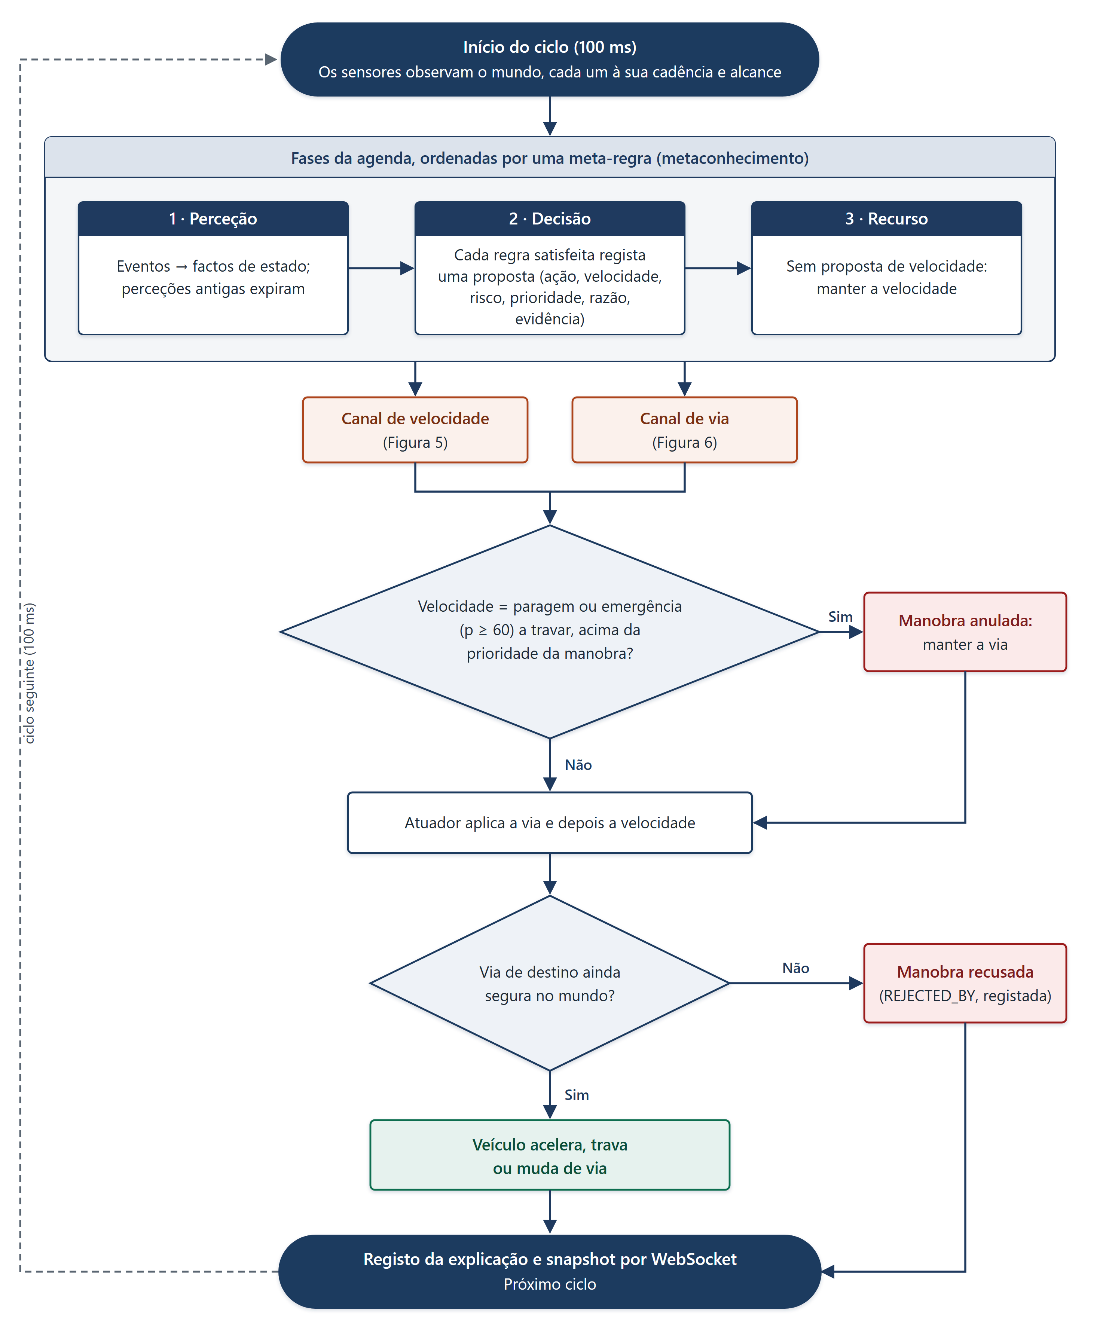
\includegraphics[width=0.79\linewidth,height=0.80\textheight,keepaspectratio]{figuras/fig04_fluxograma_de_inferencia_e}
\caption{Fluxograma de inferência e decisão em cada ciclo de 100 ms}\label{fig:4}
\end{figure}

As Figuras~\ref{fig:5} e~\ref{fig:6} detalham, para cada canal, as perguntas pela ordem de importância. A travagem de emergência está no ramo da velocidade e nunca passa pela pergunta «a manobra é permitida?».

\begin{figure}[H]
\centering
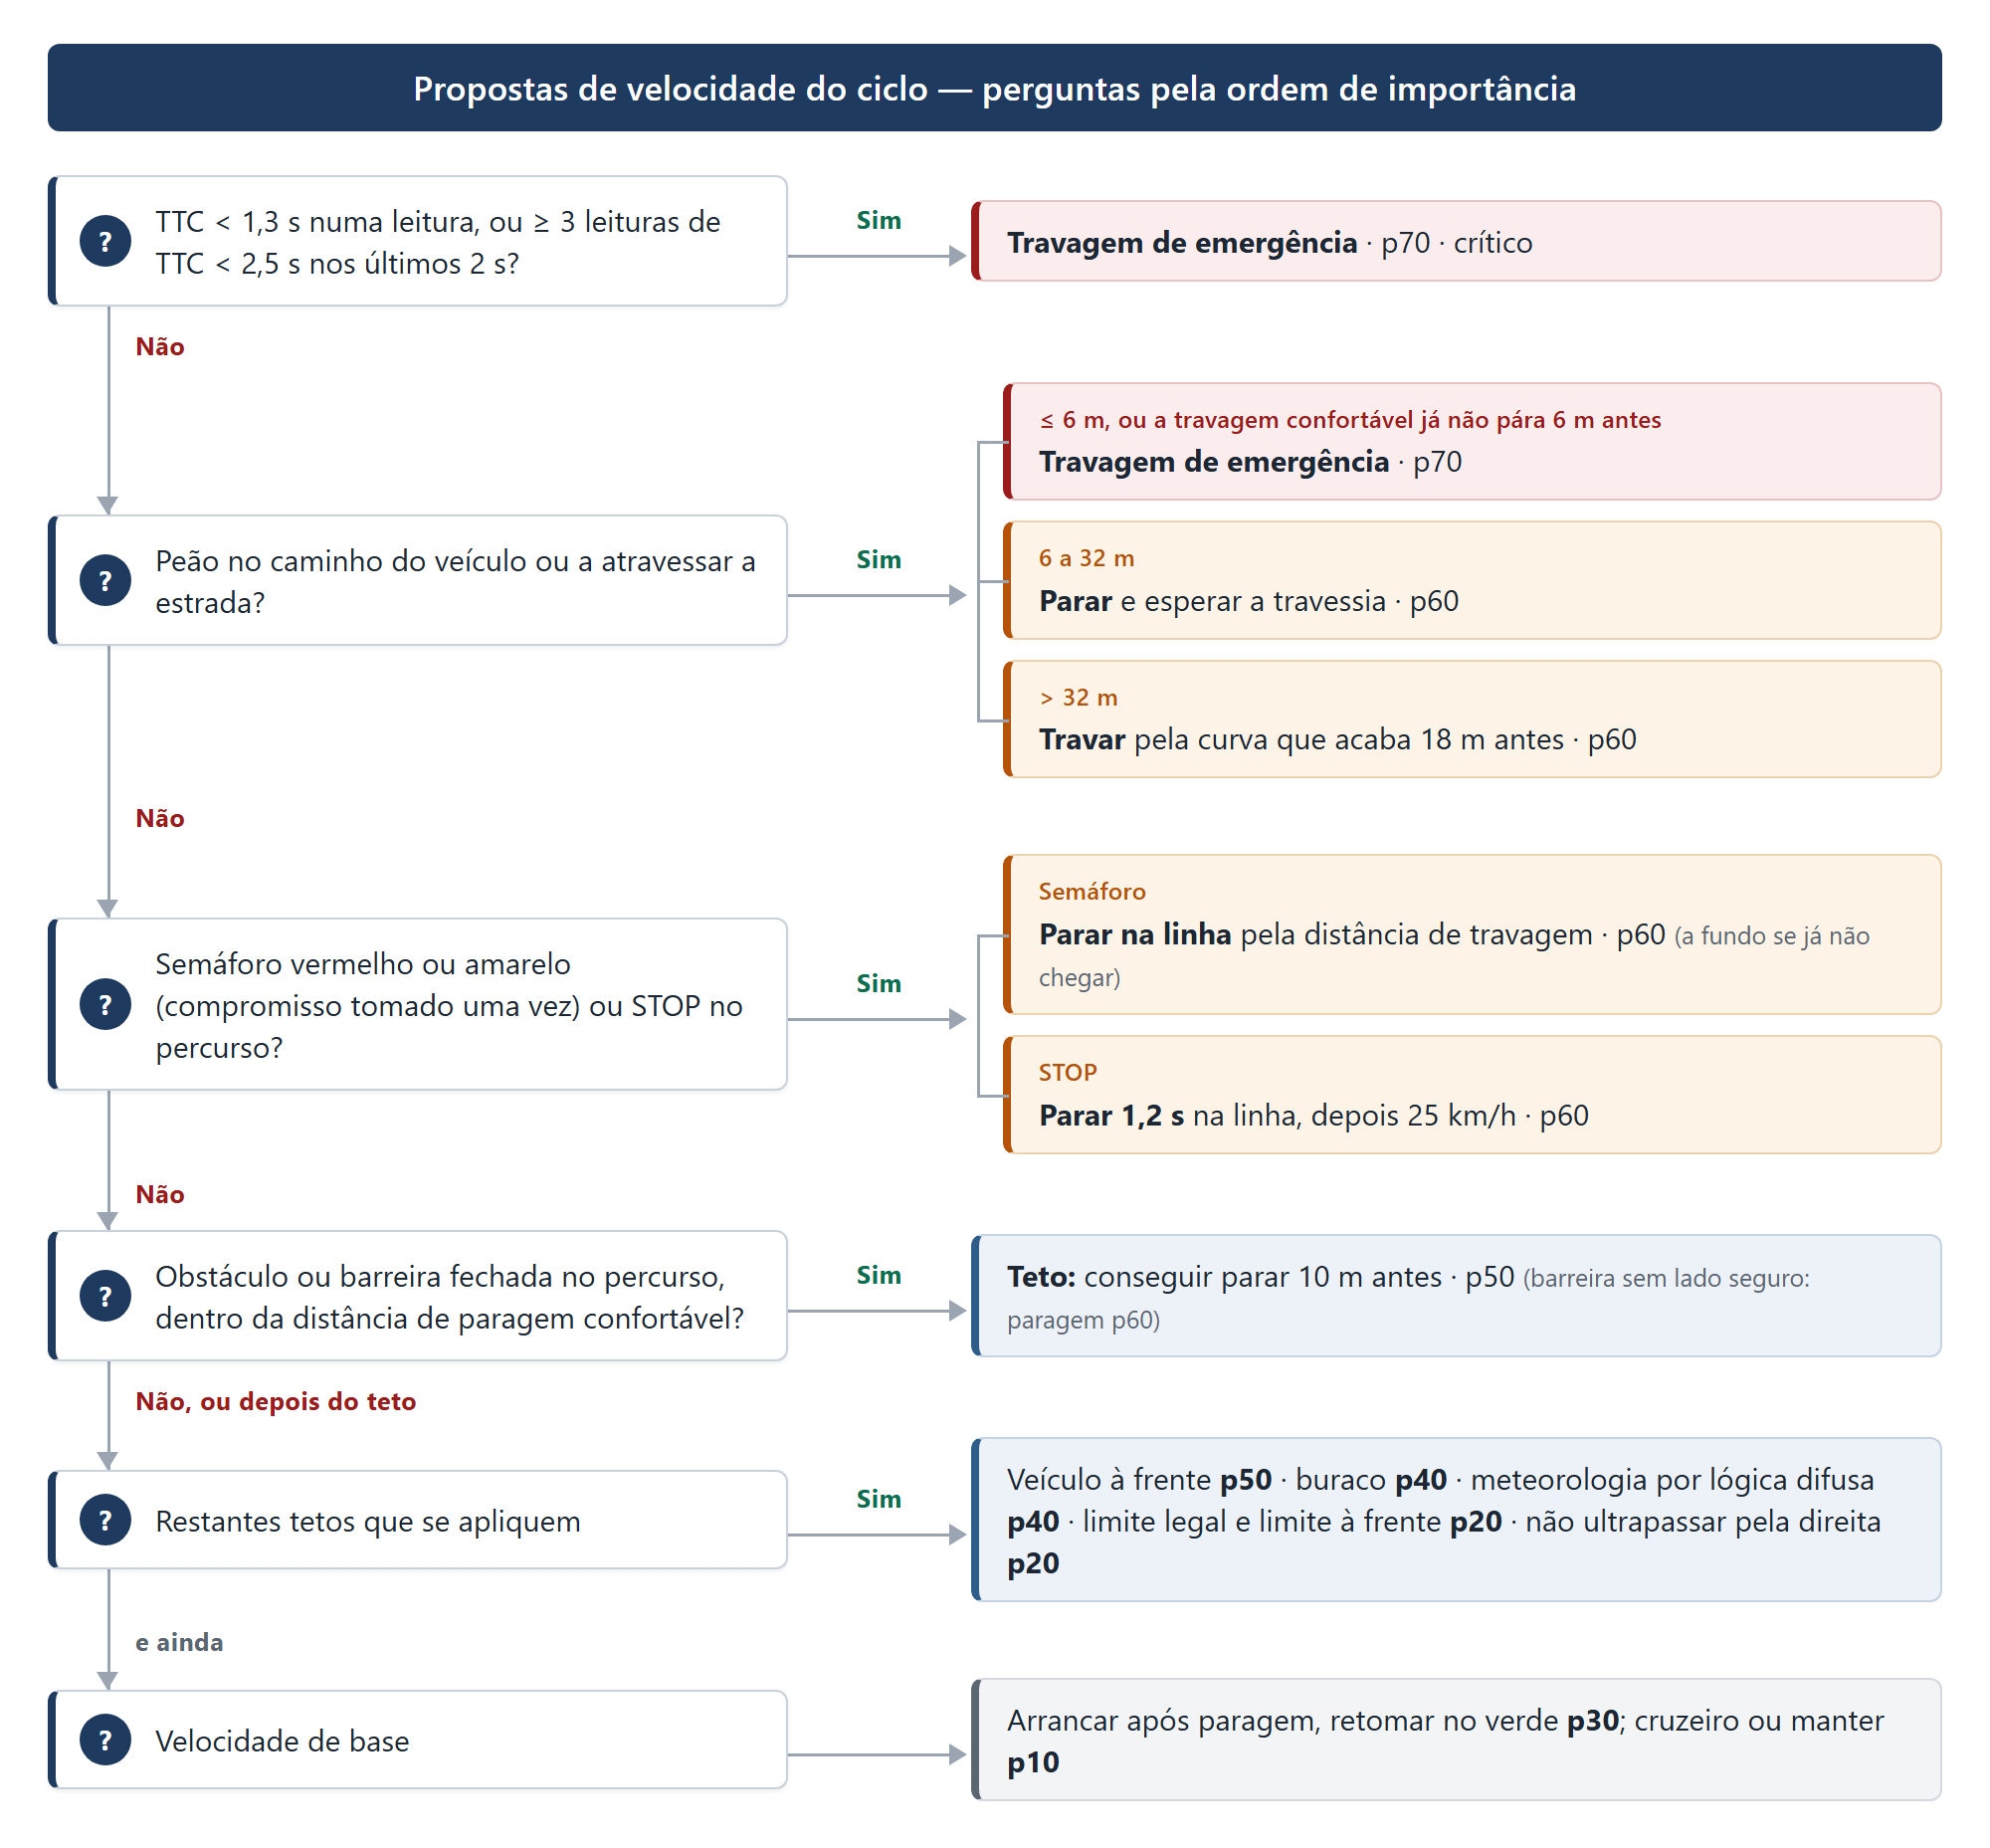
\includegraphics[width=\linewidth,height=0.80\textheight,keepaspectratio]{figuras/fig05_canal_ramo_de_velocidade}
\caption{Canal/ramo de velocidade: perguntas pela ordem de importância e decisão}\label{fig:5}
\end{figure}

No que diz respeito à arbitragem/decisão, se houver uma proposta com p>=60, vence a de maior prioridade e, em caso de empate, a de menor velocidade; um teto mais baixo limita-lhe a velocidade. Caso contrário, cumpre-se o teto mais baixo; a base só vale se nenhum teto for inferior. As restantes propostas ficam registadas como LOST\_TO.

\begin{figure}[H]
\centering
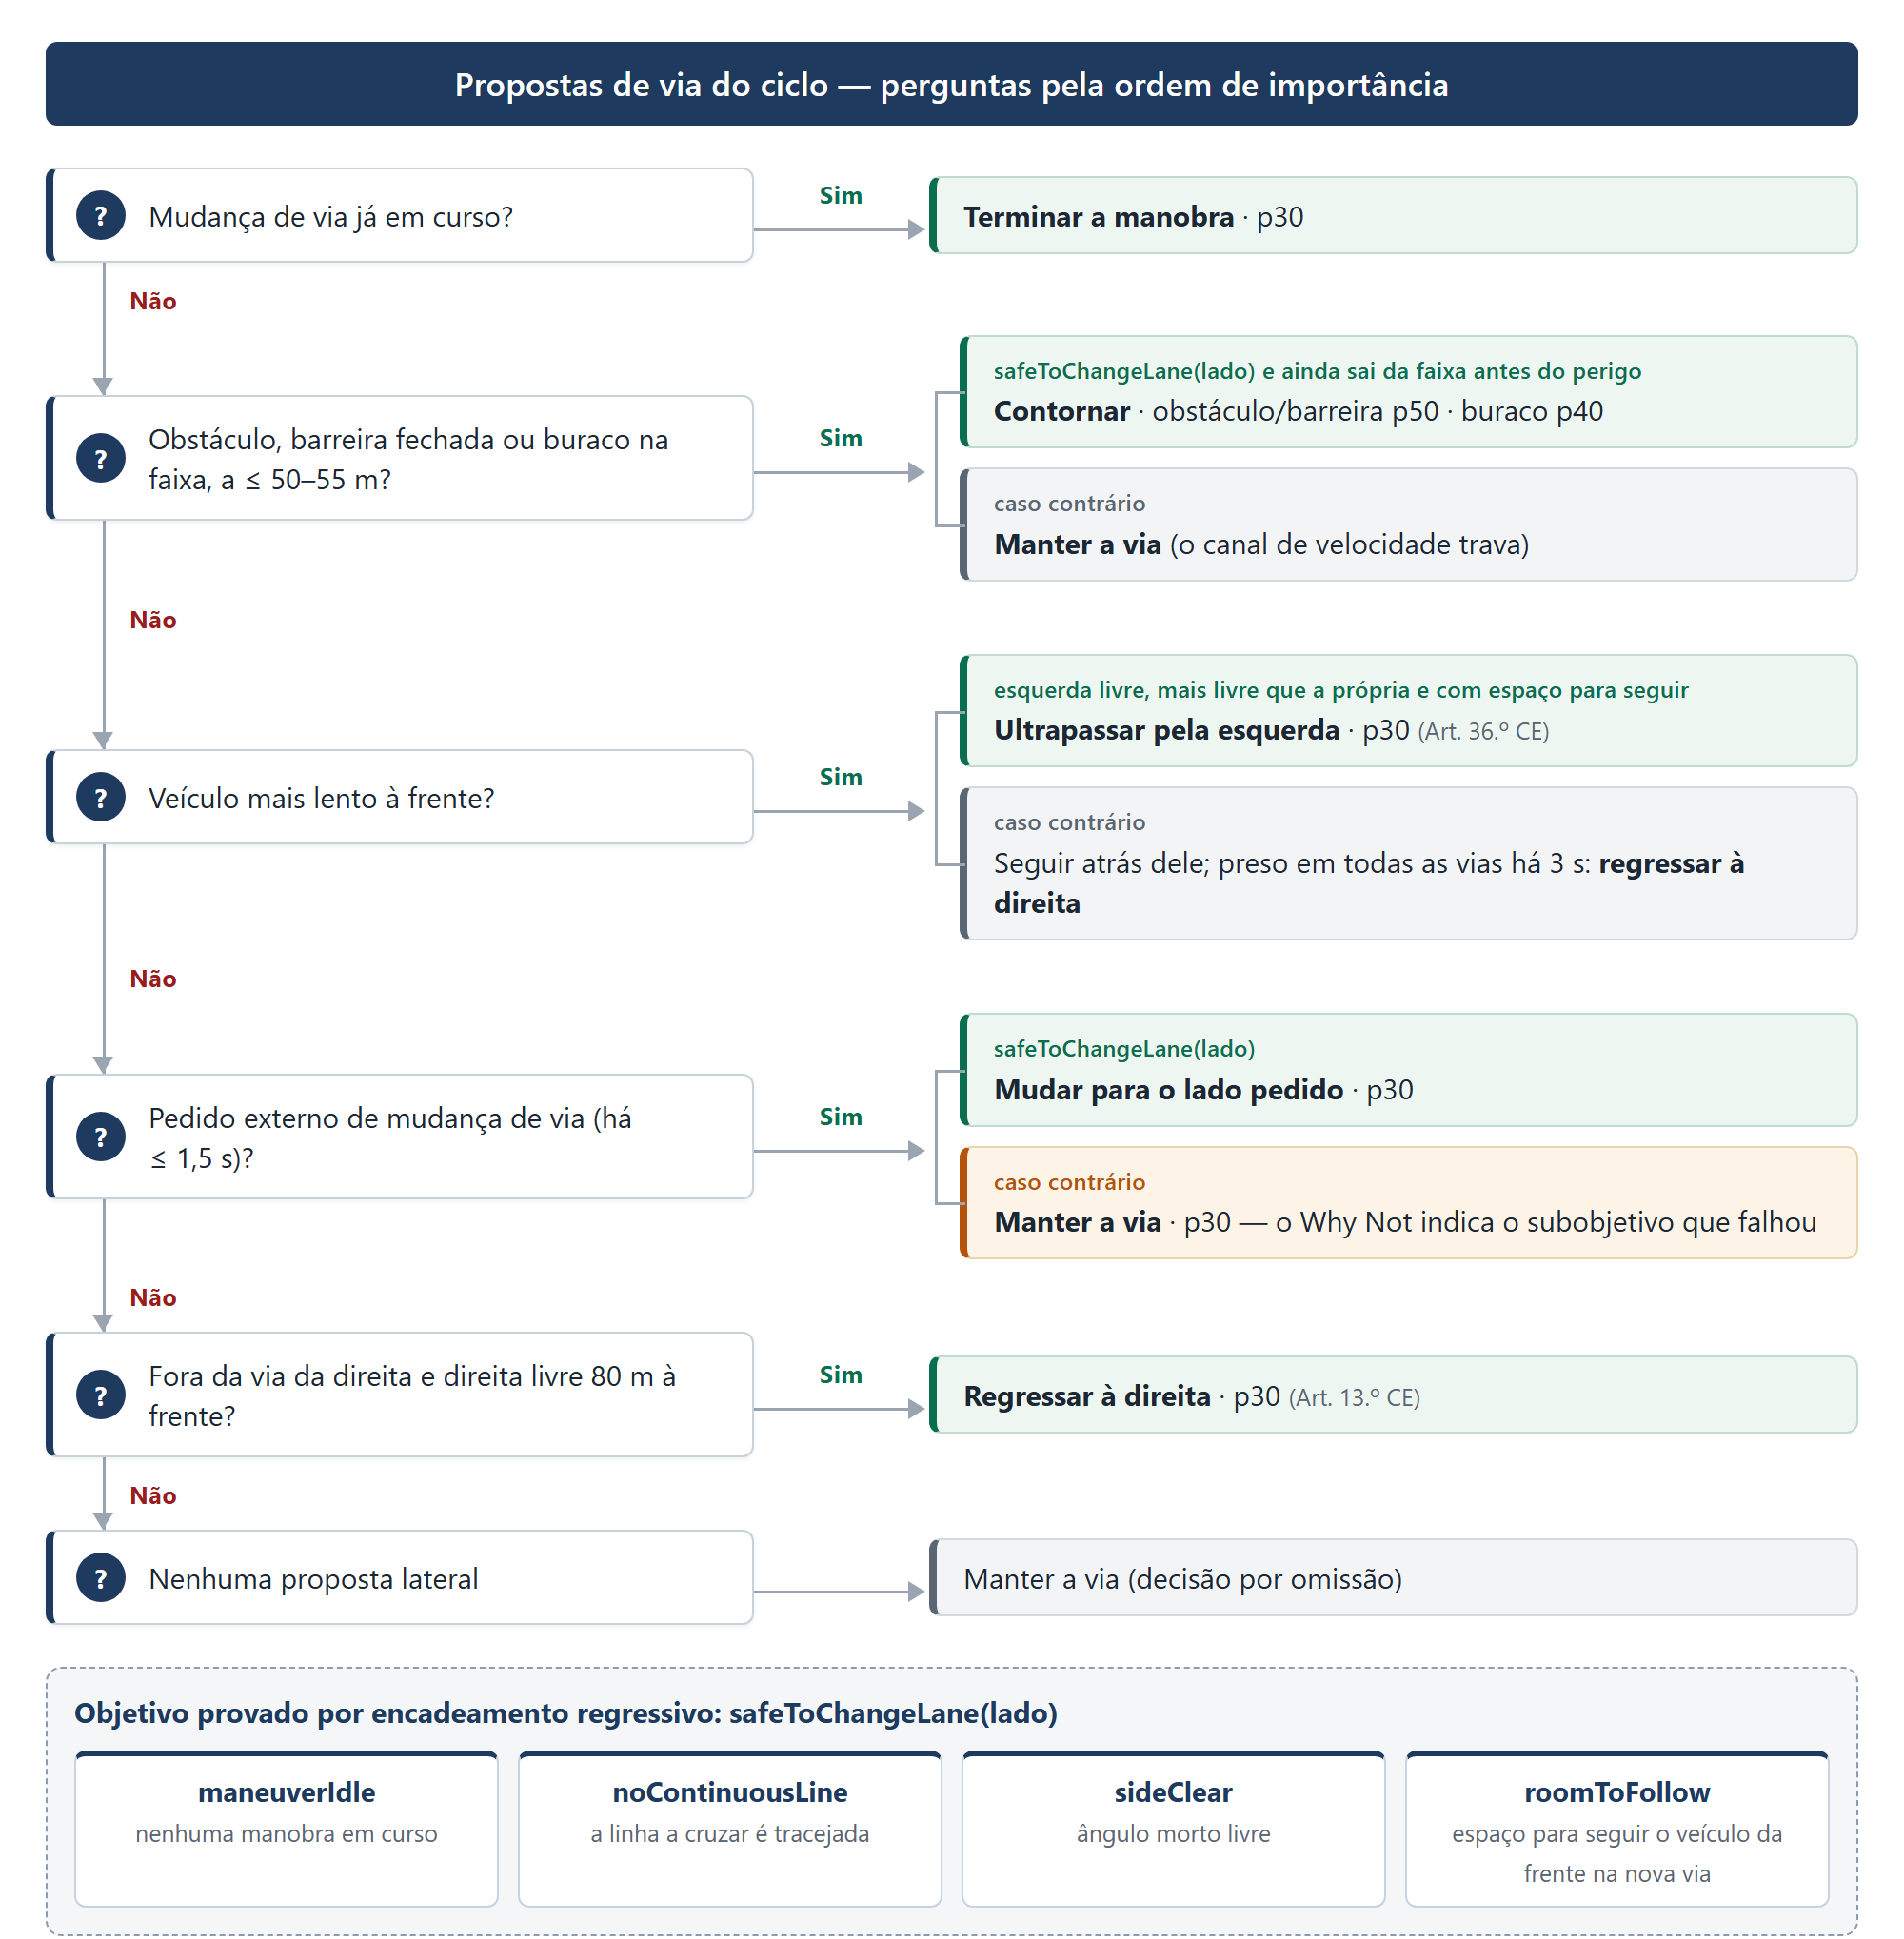
\includegraphics[width=\linewidth,height=0.80\textheight,keepaspectratio]{figuras/fig06_canal_de_via_e_objetivo_provado}
\caption{Canal de via e objetivo provado por encadeamento regressivo}\label{fig:6}
\end{figure}

O canal da via é independente do ramo de velocidade. Neste caso, em situação de empate, vence a proposta de maior prioridade, sendo que regressar à direita > mudar de via > manter a via. Uma manobra é anulada, ou seja, o veículo mantém-se na via inicial, quando a velocidade é uma paragem ou emergência a travar, de prioridade superior à da manobra.

\section{Fluxograma completo}\label{sec:5.2}

As Figuras~\ref{fig:4} a~\ref{fig:6} resumem o processo de decisão e a Figura~\ref{fig:7} apresenta o fluxograma do sistema, por inteiro, em que cada ciclo se repete por 100ms. Para facilitar a leitura, o fluxograma, foi dividido em zonas. As zonas de A a E pertencem ao ramo da velocidade e as zonas F e G ao ramo da via, e a zona G termina com a tomada de decisão.

Este fluxograma deve ser lido como uma ordem de importância e não como uma sequência de execução, uma vez que no \emph{Drools}, todas as regras cujas condições se verificam disparam no mesmo ciclo e registam a sua proposta. A decisão descrita na Secção~\ref{sec:5.1} escolhe depois a proposta vencedora. De seguida, são apresentadas as zonas A, D e G. As restantes podem ser consultadas no Anexo B.

\begin{landscape}
\begin{figure}[H]
\centering
\includegraphics[width=\linewidth,height=0.82\textheight,keepaspectratio]{figuras/fig07_fluxograma_completo_do_processo}
\caption{Fluxograma completo do processo de decisão, dividido em zonas}\label{fig:7}
\end{figure}
\end{landscape}

\textbf{Zona A – Emergência e peões (Figura~\ref{fig:12}). }É a primeira zona, porque trata as situações em que está em causa uma colisão. Uma única leitura de TTC inferior a 1,3 s, ou três leituras inferiores a 2,5 s nos últimos 2 s, dá origem a uma travagem de emergência. Se houver um peão no caminho do veículo, a resposta depende da distância. Um obstáculo grave a 8 m ou menos, na via em que o veículo circula, também dá origem a uma emergência, termina diretamente na decisão de velocidade e nunca passa por uma avaliação de manobra.

\textbf{Zona B – Semáforos (Figura~\ref{fig:13}). }Perante um semáforo vermelho, o veículo compara a distância à linha com a distância de que precisa para parar: 0,5 s de reação, mais a travagem, mais 18 m. Se estiver longe, continua. Se estiver na zona de transição, deixa de acelerar. Se já estiver dentro da distância de travagem, trava com conforto (2,8 m/s²) e para na linha, ou trava a fundo quando a travagem confortável o desloca a mais de 2 m para lá da linha. No amarelo, a decisão de parar ou prosseguir é tomada uma única vez, para evitar que o veículo hesite e trave a meio do cruzamento. No verde, o veículo segue ou volta a arrancar.\par \par \textbf{Zona C – STOP, barreiras e obstáculos (Figura~\ref{fig:14}). }No sinal STOP, o veículo para na linha e só avança, a 25 km/h, depois de estar parado pelo menos 1,2 s, o que garante a paragem completa exigida pelo Código da Estrada. Face a uma barreira fechada ou a um obstáculo dentro da distância de paragem segura, o veículo trava para conseguir parar 10 m antes. No caso da barreira, se for seguro mudar de via, essa travagem dura apenas até a mudança o tirar do caminho. Se for preciso travar a mais de 3,1 m/s², a travagem passa a ser a fundo.

\textbf{Zona D – Limites, veículo à frente e chuva (Figura~\ref{fig:15}). }Esta zona dá origem a tetos de velocidade (prioridades 50 e 20), aplicadas em simultâneo. O veículo respeita o limite em vigor e começa a abrandar a tempo de chegar ao sinal seguinte já com o novo limite, ao travar a 2,0 m/s². Com um veículo à frente, para cerca de 12 m atrás se este estiver parado. Se estiver em movimento, abranda até 3 km/h abaixo dele, acompanha a sua velocidade ou abranda apenas o necessário, conforme a distância. Com pouca aderência, essa distância duplica. O veículo não ultrapassa pela direita um veículo mais lento na via da esquerda. Com chuva, duas leituras de TTC inferiores a 3 s em 2 s levam o veículo a travar até 15 km/h.\par \textbf{Zona E – Buracos, meteorologia e velocidade de base (Figura~\ref{fig:16}). }Se não conseguir desviar-se de um buraco, o veículo passa por ele a 30 km/h, e a 20 km/h nos últimos 15 m. Junto a uma barreira aberta, não passa de 35 km/h. Com chuva, visibilidade reduzida ou pouca aderência, a lógica difusa calcula uma velocidade máxima recomendada, entre cerca de 25 e pouco mais de 70 km/h. Só depois de considerados todos os tetos é definida a velocidade de base: arrancar após uma paragem, acelerar a pedido, manter o limite do sinal ou retomar a velocidade de cruzeiro. Se nenhuma regra se aplicar, a fase de recurso mantém a velocidade. Por fim, vale a velocidade mais baixa entre a de base e todos os tetos encontrados, pelo que o veículo nunca ultrapassa o limite legal.

\textbf{Zona F – Via: obstáculos, barreiras e buracos (Figura~\ref{fig:17}). }O ramo referente ao comportamento em via começa por confirmar se uma emergência ou paragem obrigatória está a travar o veículo. Se estiver, o veículo mantém a via, o que garante que nenhuma manobra compete com uma travagem crítica. Uma mudança de via já iniciada é sempre concluída. Perante um obstáculo, uma barreira fechada ou um buraco na via, o veículo contorna-o se for seguro mudar de via e se ainda conseguir sair da via antes de lá chegar. Caso contrário, mantém a via e o canal de velocidade trata da paragem ou da passagem lenta.

\textbf{Zona G – Ultrapassagem, pedidos, regresso à direita e atuação (Figura~\ref{fig:18}). }Atrás de um veículo mais lento, o veículo ultrapassa apenas pela esquerda. Se estiver preso atrás de trânsito lento em todas as vias há pelo menos 3 s, desiste e regressa à direita. Um pedido externo de mudança de via só é aceite se a mudança for segura. Se não for, é recusado e a explicação indica qual das condições falhou. Sem outro motivo para ficar, o veículo regressa à via da direita, uma via de cada vez, como determina o Código da Estrada. As decisões de velocidade e de via juntam-se na atuação. Antes de iniciar uma mudança de via, o atuador volta a confirmar no mundo que a via de destino está livre e que não há linha contínua. Se alguma destas condições falhar, cancela a manobra e abranda 10 km/h. Por fim, ajusta a velocidade com suavidade e começa o ciclo seguinte.

\section{Explicação da decisão}\label{sec:5.3}

Cada decisão responde a três perguntas, todas a partir do que as regras registam e visíveis na interface:

\begin{itemize}
  \item \textbf{\emph{Why: }}a regra vencedora, a razão, a evidência (valores dos factos usados), o risco e a prioridade.
  \item \textbf{\emph{How:}} a linha temporal regista, com instante, cada facto inserido, atualizado ou removido e cada regra disparada, o que permite reconstruir o percurso sensor → evento → facto → regra → decisão.
  \item \textbf{\emph{Why Not: }}todas as propostas do ciclo ficam guardadas com o seu destino (Tabela~\ref{tab:9}).
\end{itemize}

\begin{tabela}{L{\dimexpr0.1865\linewidth-2\tabcolsep\relax}L{\dimexpr0.2988\linewidth-2\tabcolsep\relax}L{\dimexpr0.5128\linewidth-2\tabcolsep\relax}}
\caption{Destinos possíveis de uma proposta}\label{tab:9}\\
\linhacab \cab{\textbf{Estado}} & \cab{\textbf{Significado}} & \cab{\textbf{Exemplo}} \\
\endfirsthead
\linhacab \cab{\textbf{Estado}} & \cab{\textbf{Significado}} & \cab{\textbf{Exemplo}} \\
\endhead
WON & Venceu a arbitragem. & Travagem de emergência (p70) por TTC crítico persistente. \\
\rowcolor{corFundo}LOST\_TO & Perdeu para outra de maior prioridade. & Regras de meteorologia perdem para a emergência. \\
VETOED\_BY & Anulada por uma paragem ou emergência. & Mudança de via, anulada pela travagem de emergência. \\
\rowcolor{corFundo}CAPPED & Venceu, mas com a velocidade limitada por um teto mais baixo. & Paragem obrigatória, com outra regra a exigir velocidade ainda menor. \\
REJECTED\_BY & Recusada pelo atuador por ser insegura. & Mudança de via com a via de destino ocupada ou com linha contínua. \\
\end{tabela}

Como recomendou o perito, o texto de cada explicação é a razão e a evidência registadas pela regra que disparou, e não uma descrição escrita à parte. No fim da viagem a sessão é gravada em JSON, e qualquer decisão pode ser questionada depois sem reavaliar nada. A Secção~\ref{sec:6.4} mostra as três explicações num caso concreto.

% ---------------------------------------------------------------
% seccoes/implementacao.tex — Implementação
% ---------------------------------------------------------------

\chapter{Implementação}\label{sec:6}

\section{Arquitetura}\label{sec:6.1}

A arquitetura utilizada teve como foco separar o mundo simulado, a perceção e o conhecimento (Figura~\ref{fig:8}). O \cod{WorldState} contém tudo o que existe no cenário, mas o motor de inferência só conhece o que os sensores detetaram. Toda a política de decisão está nas regras; o código Java simula, encaminha eventos e aplica decisões. Por sua vez, a interface apenas apresenta a informação e envia comandos. A Tabela~\ref{tab:10} apresenta os principais componentes, com base nos seguintes princípios:

\begin{itemize}
  \item A cada 100 ms é executado um ciclo;
  \item todos os pedidos REST passam por métodos sincronizados do SimulationEngine
  \item Comandos por REST, estado por WebSocket. Cada pedido tem a sua resposta; o estado completo é enviado para o \emph{browser} a cada ciclo.
\end{itemize}

\begin{figure}[H]
\centering
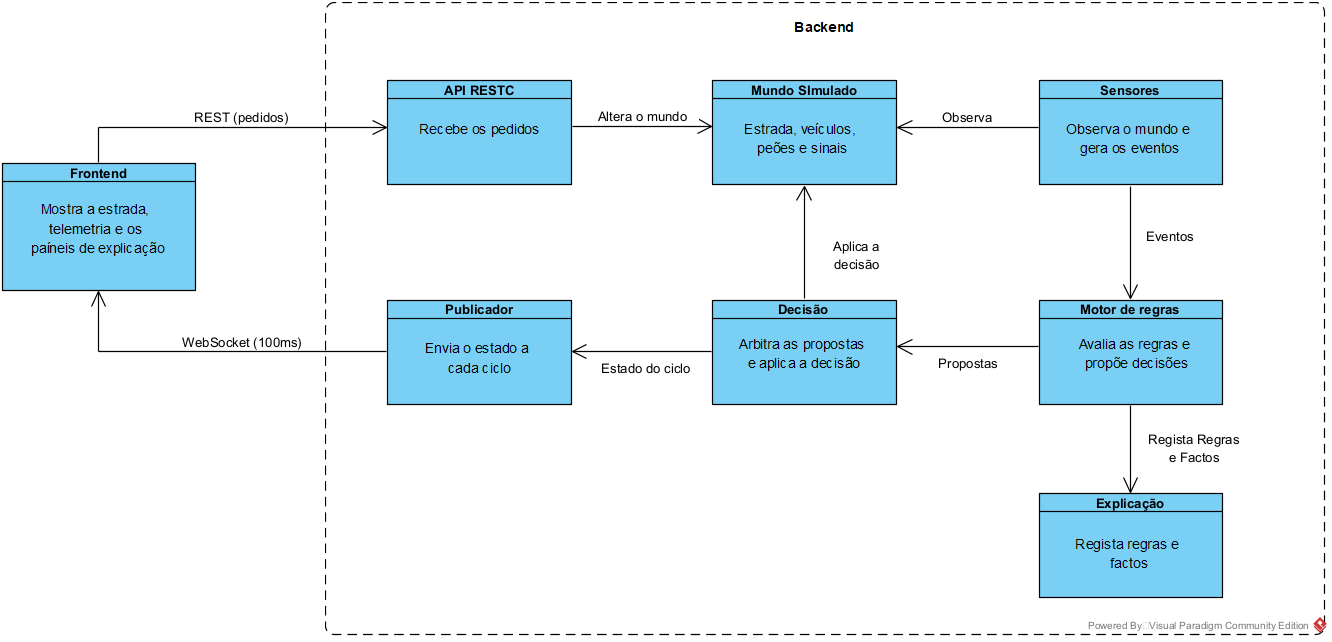
\includegraphics[width=\linewidth,height=0.80\textheight,keepaspectratio]{figuras/fig08_arquitetura_do_sistema_e_fluxo}
\caption{Arquitetura do sistema e fluxo de informação}\label{fig:8}
\end{figure}

\begin{tabela}{L{\dimexpr0.1797\linewidth-2\tabcolsep\relax}L{\dimexpr0.2994\linewidth-2\tabcolsep\relax}L{\dimexpr0.5189\linewidth-2\tabcolsep\relax}}
\caption{Tecnologias utilizadas}\label{tab:10}\\
\linhacab \cab{\textbf{Componente}} & \cab{\textbf{Tecnologia}} & \cab{\textbf{Utilização}} \\
\endfirsthead
\linhacab \cab{\textbf{Componente}} & \cab{\textbf{Tecnologia}} & \cab{\textbf{Utilização}} \\
\endhead
Backend & Java 17, Spring Boot 3.3.4 & Simulação, sensores, motor de inferência e API REST/WebSocket \\
\rowcolor{corFundo}Motor de regras & Drools / KIE 8.44 & Sessão com estado, regras DRL, CEP, encadeamento progressivo e consultas \\
Frontend & Angular 18, RxJS & Visualização da simulação e dos painéis do sistema pericial \\
\rowcolor{corFundo}Comunicação & WebSocket e REST & Estado em tempo real (WebSocket) e pedidos (REST) \\
Testes & JUnit 5, Jasmine/Karma, Playwright & Regras, arbitragem, ciclo de simulação, integração e testes de ponta a ponta \\
\end{tabela}

\section{O ciclo de simulação e organização do motor de inferência}\label{sec:6.2}

O ciclo de simulação tem por base intervalos de 100 ms, durante os quais são processadas as leituras dos sensores simulados, atualizada a informação disponível na memória de trabalho e avaliadas as regras aplicáveis. As decisões resultantes são utilizadas para atualizar o estado do veículo simulado, o que permite que as alterações do ambiente sejam consideradas nos ciclos seguintes, como representado na Figura~\ref{fig:9}, através da sequência das operações realizadas em cada ciclo.

\begin{figure}[H]
\centering
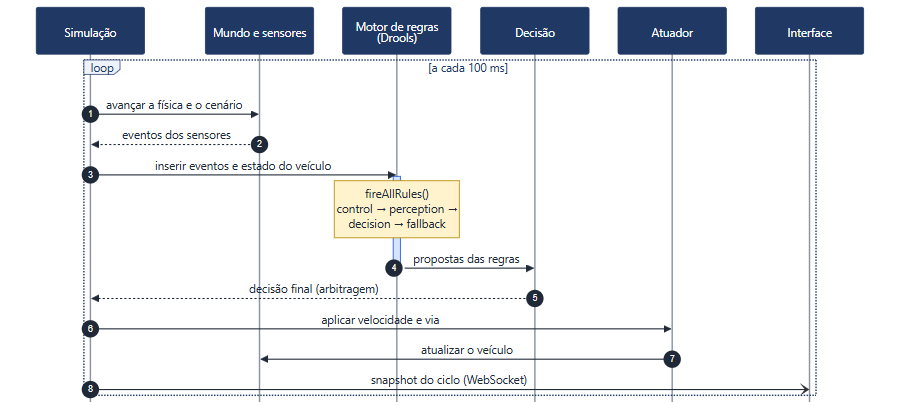
\includegraphics[width=0.94\linewidth,height=0.80\textheight,keepaspectratio]{figuras/fig09_sequencia_de_um_ciclo_de}
\caption{Sequência de um ciclo de simulação}\label{fig:9}
\end{figure}

Com o objetivo de organizar a informação recebida pelo motor de inferência \emph{Drools}, os eventos são encaminhados através de seis entry points, apresentados na Tabela~\ref{tab:11}. Esta organização permite separar os diferentes tipos de informação e identificar os fluxos relevantes para a avaliação das regras, incluindo aquelas que dependem de condições temporais.

\begin{tabela}{L{\dimexpr0.2852\linewidth-2\tabcolsep\relax}L{\dimexpr0.7128\linewidth-2\tabcolsep\relax}}
\caption{Entry points e eventos}\label{tab:11}\\
\linhacab \cab{\textbf{Entry point}} & \cab{\textbf{Eventos}} \\
\endfirsthead
\linhacab \cab{\textbf{Entry point}} & \cab{\textbf{Eventos}} \\
\endhead
VEHICLE\_STREAM & Velocidade do veículo \\
\rowcolor{corFundo}PERCEPTION\_STREAM & Distância, velocidade relativa e TTC; peões; ocupação das vias laterais; veículos nas vias vizinhas \\
ROAD\_STREAM & Sinais de limite de velocidade e de STOP, passadeiras, buracos, obstáculos, barreiras \\
\rowcolor{corFundo}TRAFFIC\_STREAM & Estado dos semáforos \\
ENVIRONMENT\_STREAM & Chuva, visibilidade e aderência \\
\rowcolor{corFundo}COMMAND\_STREAM & Pedidos de aceleração e de mudança de via \\
\end{tabela}

As regras são organizadas em quatro grupos, apresentados na Tabela~\ref{tab:12}. Esta divisão permite separar o processamento das perceções, a avaliação das condições de decisão e os comportamentos predefinidos quando nenhuma outra ação é proposta. A sequência de execução é coordenada por uma meta-regra de controlo, através da qual é estabelecida uma ordem entre as diferentes fases do processo de inferência.

\begin{tabela}{L{\dimexpr0.1496\linewidth-2\tabcolsep\relax}L{\dimexpr0.1398\linewidth-2\tabcolsep\relax}L{\dimexpr0.7086\linewidth-2\tabcolsep\relax}}
\caption{Grupos de agenda}\label{tab:12}\\
\linhacab \cab{\textbf{Grupo}} & \cab{\textbf{Nº de Regras}} & \cab{\textbf{Função}} \\
\endfirsthead
\linhacab \cab{\textbf{Grupo}} & \cab{\textbf{Nº de Regras}} & \cab{\textbf{Função}} \\
\endhead
control & 1 & Meta-regra responsável por coordenar a sequência de execução dos grupos de agenda \\
\rowcolor{corFundo}perception & 33 & Transformação de eventos em factos de estado, gestão da validade das perceções e avaliação da segurança das vias adjacentes \\
decision & 87 & Avaliação das condições e proposta de ações, assim como o tratamento das condições meteorológicas, o arranque e a ultrapassagem \\
\rowcolor{corFundo}fallback & 2 & Definição de comportamentos predefinidos quando não existem outras decisões aplicáveis \\
\end{tabela}

No que diz respeito ao tratamento das condições meteorológicas, é utilizada a lógica difusa para representar grandezas como a visibilidade e a aderência, na qual cada leitura pertence, com um grau entre 0 e 1, a vários conjuntos ao mesmo tempo, nomeadamente:

\begin{itemize}
  \item Conjuntos difusos: a visibilidade e a aderência partilham quatro conjuntos linguísticos, designados por fraca, reduzida, razoável e boa (Figura~\ref{fig:10}a). Os conjuntos sobrepõem-se e, em qualquer ponto, os graus de pertença somam 1, pelo que uma leitura pode ser, por exemplo, razoável com grau de 0,75 e reduzida com grau 0,25. A saída é a velocidade máxima recomendada, descrita por cinco conjuntos: muito lenta, lenta, moderada, prudente e ligeira (Figura~\ref{fig:10}b).
\end{itemize}

\begin{figure}[H]
\centering
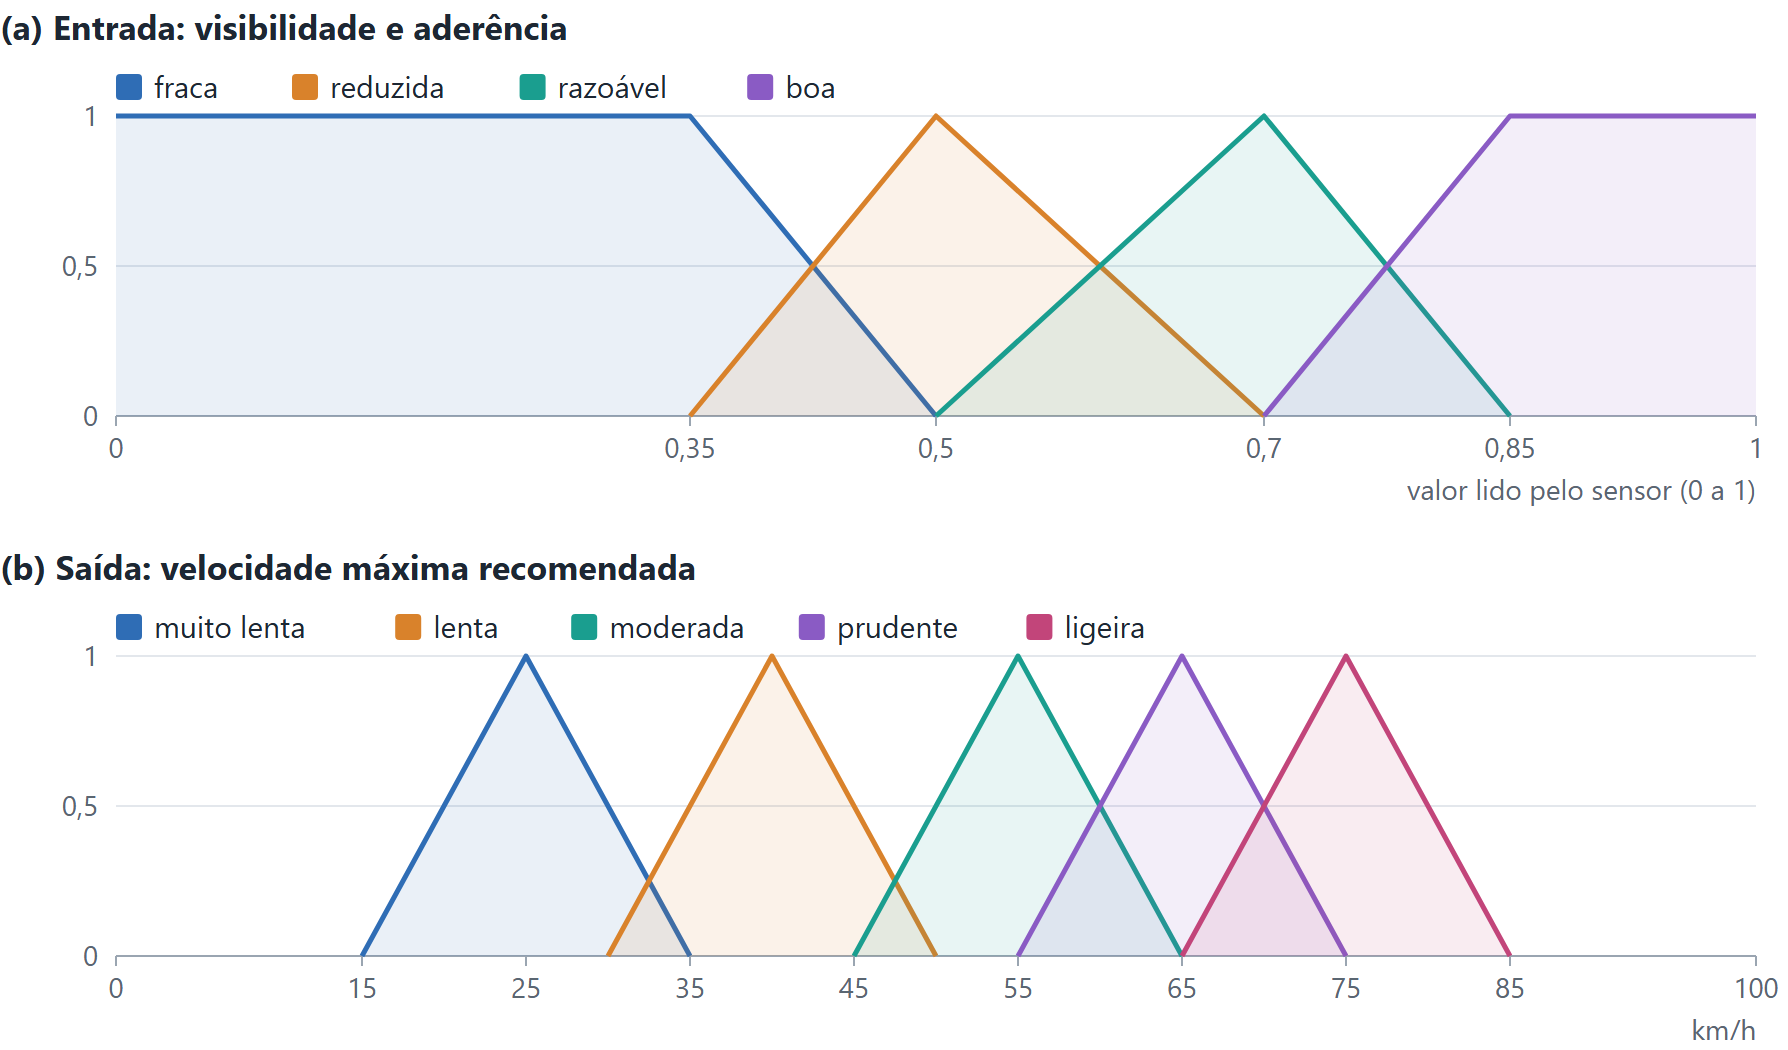
\includegraphics[width=0.89\linewidth,height=0.80\textheight,keepaspectratio]{figuras/fig10_conjuntos_difusos_a_visibilidade}
\caption{Conjuntos difusos: (a) visibilidade e aderência e (b) velocidade máxima recomendada}\label{fig:10}
\end{figure}

\begin{itemize}
  \item Regras difusas: As duas grandezas são combinadas, através de cinco regras (Tabela~\ref{tab:13}). As três primeiras utilizam a disjunção (OU), calculada pelo máximo, uma vez que basta uma das grandezas estar degradada para justificar a redução da velocidade. As duas últimas utilizam a conjunção (E), calculada pelo mínimo, e aplicam-se apenas quando ambas são boas, situação em que a chuva distingue uma velocidade prudente de uma velocidade ligeira.
\end{itemize}

\begin{tabela}{L{\dimexpr0.0924\linewidth-2\tabcolsep\relax}L{\dimexpr0.5482\linewidth-2\tabcolsep\relax}L{\dimexpr0.3574\linewidth-2\tabcolsep\relax}}
\caption{Regras difusas da meteorologia}\label{tab:13}\\
\linhacab \cab{\textbf{Regra}} & \cab{\textbf{SE}} & \cab{\textbf{ENTÃO velocidade}} \\
\endfirsthead
\linhacab \cab{\textbf{Regra}} & \cab{\textbf{SE}} & \cab{\textbf{ENTÃO velocidade}} \\
\endhead
1 & visibilidade fraca OU aderência fraca & muito lenta \\
\rowcolor{corFundo}2 & visibilidade reduzida OU aderência reduzida & lenta \\
3 & visibilidade razoável OU aderência razoável & moderada \\
\rowcolor{corFundo}4 & chuva E visibilidade boa E aderência boa & prudente \\
5 & sem chuva E visibilidade boa E aderência boa & ligeira \\
\end{tabela}

\begin{itemize}
  \item Aplicação no Drools: Uma vez que o Drools não tem suporte nativo para a lógica difusa, o controlador foi implementado através das regras do grupo \emph{decision}, com o apoio da classe \emph{FuzzySupport}. A fuzzificação converte as leituras em graus de pertença, que são, posteriormente, utilizados pelas regras para produzir as conclusões difusas. Tanto os graus de pertença como as conclusões são inseridos através do \emph{insertLogical}, o que permite ao \emph{Drools} removê-los automaticamente quando as leituras meteorológicas mudam. A título de exemplo, com chuva, visibilidade de 0,7 e aderência de 0,65, a visibilidade é razoável com grau 1 e a aderência é razoável com grau 0,75 e reduzida com grau 0,25. Assim, a regra 3 dispara com grau 1, conclui com velocidade moderada, e a regra 2 com grau 0,25, conclui com velocidade lenta. O centroide da área resultante é de 50,6 km/h, ou seja, aproximadamente 51 km/h, um valor próximo da velocidade moderada, mas reduzido pela contribuição da velocidade lenta (Figura~\ref{fig:11}).
\end{itemize}

\begin{figure}[H]
\centering
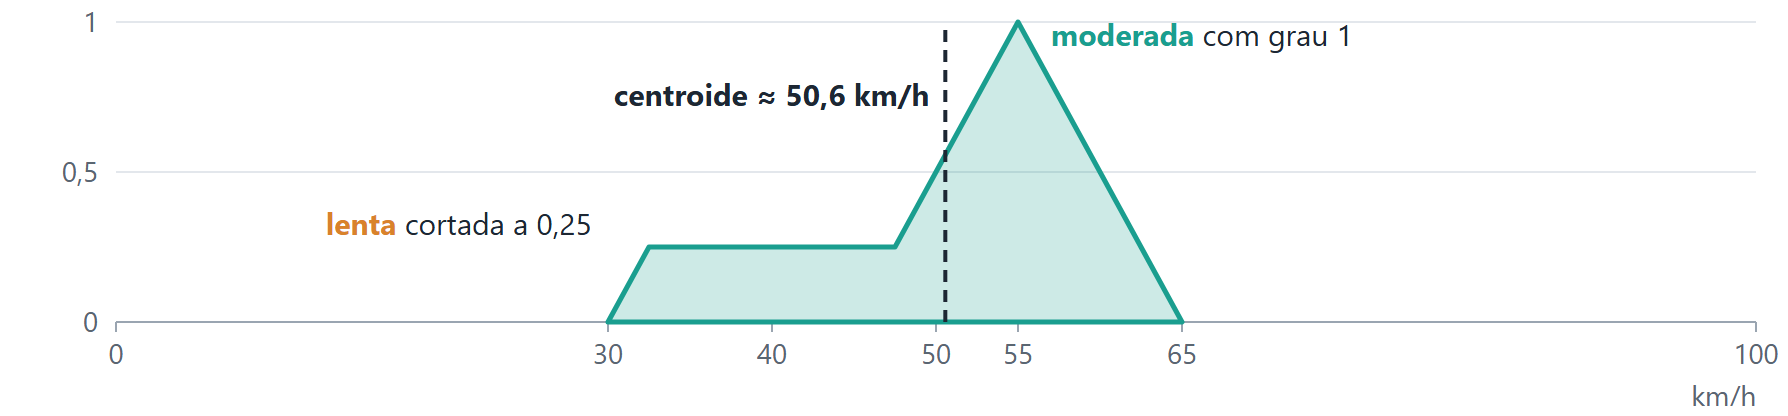
\includegraphics[width=0.89\linewidth,height=0.80\textheight,keepaspectratio]{figuras/fig11_exemplo_com_chuva_visibilidade_0}
\caption{Exemplo com chuva, visibilidade 0,7 e aderência 0,65}\label{fig:11}
\end{figure}

Desta forma, a organização dos fluxos e dos grupos permite estruturar o processo de inferência, enquanto a utilização das regras temporais e difusas possibilita considerar a evolução das condições observadas durante a simulação.

\section{Comunicação em tempo real: WebSocket}\label{sec:6.3}

A interface tem de mostrar, dez vezes por segundo, o veículo, as deteções, as decisões de velocidade e de via, a linha temporal e a memória de trabalho. Para isso, o backend mantém uma ligação WebSocket com o browser e envia, a cada ciclo, um snapshot JSON completo do sistema, num só sentido, do backend para o frontend. Como o snapshot inclui a decisão, as propostas, a evidência, a memória de trabalho e a linha temporal, a explicação de cada ciclo chega à interface sem cálculo adicional. Os comandos seguem por REST, porque cada um precisa da sua própria resposta e código de erro, e o backend envia um snapshot logo a seguir a cada comando, para que o efeito seja visível sem esperar pelo ciclo seguinte (Tabela~\ref{tab:14}). A ligação só é aceite a partir da origem da interface do projeto; as restantes são rejeitadas (403).

\begin{tabela}{L{\dimexpr0.5267\linewidth-2\tabcolsep\relax}L{\dimexpr0.4713\linewidth-2\tabcolsep\relax}}
\caption{Canais de comunicação}\label{tab:14}\\
\linhacab \cab{\textbf{Função}} & \cab{\textbf{Canal}} \\
\endfirsthead
\linhacab \cab{\textbf{Função}} & \cab{\textbf{Canal}} \\
\endhead
Ciclo de vida (iniciar, pausar, parar, reiniciar) & REST \\
\rowcolor{corFundo}Carregar cenários & REST \\
Alterar o mundo (elementos, meteorologia) & REST \\
\rowcolor{corFundo}Consultar viagens e perguntas Why / Why Not / How & REST \\
Estado em tempo real & WebSocket \\
\end{tabela}

A publicação do estado não pode atrasar a inferência. Por isso, cada cliente tem um emissor próprio e uma única posição de espera, que guarda apenas o snapshot mais recente: um browser lento salta estados intermédios, mas como cada snapshot é completo nunca fica com informação errada, e o ciclo de 100 ms mantém-se inalterado. Se a ligação falhar, o frontend deteta a falha e restabelece-a automaticamente.

\section{Cenários}\label{sec:6.4}

Foram definidos cenários pré-construídos que abrangessem um pouco de todo o sistema. Neste sentido, a título de exemplo, apresenta-se a traçagem do cenário de TTC crítico com chuva, na Tabela~\ref{tab:15}. Para este cenário considera-se que o veículo segue a 95 km/h na via do meio, com outro a 30 km/h 40 m à frente (TTC ≈ 2,2 s).

\begin{tabela}{L{\dimexpr0.0741\linewidth-2\tabcolsep\relax}L{\dimexpr0.3513\linewidth-2\tabcolsep\relax}L{\dimexpr0.1671\linewidth-2\tabcolsep\relax}L{\dimexpr0.2078\linewidth-2\tabcolsep\relax}L{\dimexpr0.1977\linewidth-2\tabcolsep\relax}}
\caption{Traçagem do cenário TTC crítico com chuva}\label{tab:15}\\
\linhacab \cab{t} & \cab{Perceção e estado} & \multicolumn{2}{L{\dimexpr0.3749\linewidth-2\tabcolsep\relax}}{\cab{Propostas de decisão}} & \cab{Decisão aplicada} \\
\endfirsthead
\linhacab \cab{t} & \cab{Perceção e estado} & \multicolumn{2}{L{\dimexpr0.3749\linewidth-2\tabcolsep\relax}}{\cab{Propostas de decisão}} & \cab{Decisão aplicada} \\
\endhead
0,1 s & 1.ª leitura de TTC: ainda não há janela; lógica difusa (Mamdani) com insertLogical dá ≈ 51 km/h & \textbf{WON} & Keep safe following distance...: 48 km/h · p50. & Vence o teto mais baixo;\par a ultrapassagem inicia-se \\*
 &  & \textbf{LOST\_TO} & Defuzzify weather speed ceiling: 51 km/h · p40. &  \\*
 &  & \textbf{WON} & Overtake slow front vehicle via left lane · p30 &  \\
\rowcolor{corFundo}0,2 s & 2 leituras de TTC < 3 s em 2 s, cada uma coincide[400ms] com uma leitura de chuva & \textbf{WON} & Persistent low TTC in rain increases conservatism: BRAKE 15 km/h · p50 & \textbf{Trava; }\par \textbf{manobra em curso} \\
0,3 s & accumulate ... over window.time(2s): 3 leituras de TTC < 2,5 s (mínimo 1,94 s) & \textbf{WON} & Emergency brake when persistent TTC is critical · p70. & \textbf{−8,5 m/s² e luzes de emergência; }\par \textbf{a manobra já iniciada não é abortada} \\*
 &  & \textbf{LOST\_TO} & chuva, seguimento, aproximação, difusa, cruzeiro &  \\*
 &  & \textbf{VETOED\_BY} & Maintain ongoing lane change left (anulada) &  \\
\rowcolor{corFundo}3,1 s & Manobra concluída: via da esquerda, sem veículo à frente & \textbf{WON} & Defuzzify weather speed ceiling: 51 km/h · p40 & Acelera de 10 até ≈ 51 km/h \\
\end{tabela}

% ---------------------------------------------------------------
% seccoes/ponto_situacao.tex — Ponto de situação
% ---------------------------------------------------------------

\chapter{Ponto de situação}\label{sec:7}

\section{Adequação ao meio ambiente, empresas e organizações}\label{sec:7.1}

O principal valor do sistema está na explicabilidade: cada decisão fica ligada à regra que a originou, aos factos usados e às alternativas rejeitadas. Isto interessa a quem tem de desenvolver, testar e justificar sistemas de condução autónoma. Os fabricantes e fornecedores de software automóvel poderão usá-lo como apoio às equipas de engenharia em testes preliminares em simulação, para perceber porque o sistema decidiu de determinada forma e, potencialmente, reduzir o recurso a ensaios físicos. As empresas de simulação e validação poderão integrá-lo como módulo complementar que explica e rastreia as decisões nos resultados dos testes, e os centros de investigação e universidades como plataforma para projetos de sistemas periciais e de IA explicável.

Fora do setor automóvel, a mesma abordagem pode aplicar-se à robótica móvel e à automação industrial, com as devidas adaptações. Sendo um protótipo académico, com sensores e ambiente simulados, qualquer utilização real exigiria integração com sensores reais e validação em ambientes mais realistas.

\section{Restrições e limitações}\label{sec:7.2}

Apesar dos resultados obtidos, importa reconhecer algumas restrições e limitações associadas ao desenvolvimento e funcionamento do sistema. Estas resultam tanto de decisões tomadas para delimitar o âmbito do projeto como de simplificações do ambiente de simulação e de aspetos identificados durante a implementação e validação.

No que diz respeito à simulação de cenários, embora o ambiente apresente uma representação visual em 3D, utiliza modelos simplificados da estrada, do comportamento dos veículos e das condições de circulação, limitado a três vias de trânsito. O âmbito do projeto exclui ainda o planeamento de percursos, a circulação em sentido contrário, os ciclistas, o estado do condutor e o controlo detalhado da dinâmica do veículo.

Relativamente à perceção do ambiente, os sensores simulados apresentam algumas simplificações, nomeadamente a existência de ruído apenas no radar, sem situações de informação contraditória entre sensores. No que respeita ao funcionamento do sistema, a necessidade de executar ciclos de decisão a cada 100 ms condicionou a complexidade do processamento, tendo sido estabelecido um limite máximo de 5000 disparos de regras por ciclo como medida de proteção. Foram também identificadas limitações na gestão de algumas decisões, nomeadamente a possibilidade de uma ordem de paragem perante um peão se sobrepor a uma travagem de emergência necessária devido a um obstáculo mais próximo, uma vez que ambas estabelecem uma velocidade de destino de 0 km/h. Adicionalmente, as mudanças de via seguem um modelo simplificado que não permite cancelar uma manobra depois de iniciada, mesmo perante alterações das condições de circulação.

Quanto à aquisição de conhecimento, o contacto com o perito deu-se quando o desenvolvimento do projeto já se encontrava em curso, embora numa fase inicial. Foram realizadas várias sessões de esclarecimento para apoiar a construção da base de conhecimento e, após a conclusão do desenvolvimento, o sistema foi apresentado ao perito para apreciação.

Por fim, a validação foi realizada através de cenários simulados e testes automáticos, não tendo sido considerados testes com veículos reais. Acresce que o simulador não dispõe de um mecanismo automático de deteção de colisões, sendo necessário recorrer a testes que verifiquem explicitamente a ocorrência de embates. Assim, os resultados obtidos permitem avaliar o funcionamento do sistema nos cenários considerados, mas não garantem o seu comportamento em condições reais de circulação.

Estas restrições e limitações não comprometem os objetivos definidos para o projeto, mas identificam oportunidades de desenvolvimento futuro, nomeadamente ao nível da consistência das decisões, da segurança das manobras e da aproximação do sistema a condições reais de condução.

\section{Possibilidades de desenvolvimento futuro}\label{sec:7.3}

As possibilidades de evolução decorrem destas limitações identificadas e das indicações do perito após a apresentação do resultado final, nomeadamente:

\begin{itemize}
  \item Fiabilidade dos sensores: associar um nível de confiança a cada deteção, confirmar deteções entre câmara e radar, acrescentar o LiDAR como terceira fonte em caso de divergência [10, 11, 12] e parar de forma controlada perante a falha de um sensor, como indicou o perito;
  \item Interação entre veículos\textbf{:} usar a Teoria dos Jogos para escolher entre manobras já provadas seguras quando a decisão depende do comportamento esperado de outros condutores, mantendo as regras de segurança como restrições;
  \item Domínio: cruzamentos e prioridade, trânsito em sentido contrário, ciclistas, intervalo temporal (THW) e saída involuntária da via;
  \item Integração: ligar a camada de decisão a um simulador de condução mais realista e, depois, a dados de sensores reais;
\end{itemize}

% ---------------------------------------------------------------
% seccoes/conclusao.tex — Conclusão
% ---------------------------------------------------------------

\chapter{Conclusão}\label{sec:8}

Em resposta à questão central apresentada na Secção~\ref{sec:1.2}, o trabalho desenvolvido demonstra que é possível utilizar um motor de regras associado ao processamento de eventos complexos para apoiar a tomada de decisão de um veículo, em tempo real, a partir de dados provenientes de sensores com diferentes frequências de atualização. Para tal, foi fundamental estruturar o processo de decisão em três etapas distintas: perceção, geração de propostas e decisões.

A base de conhecimento, construída com base na regulamentação rodoviária, na literatura e no contributo do perito do domínio, integra um conjunto de regras distintas e contempla cenários predefinidos de condução. A combinação do raciocínio temporal e da lógica difusa permitiu abordar diferentes situações de circulação e incorporar distintas formas de raciocínio no processo de decisão. A distinção entre risco e prioridade, aliada à decisão em duas vertentes (velocidade e via), permite que a escolha das ações não dependa da ordem de execução das regras.

Neste sentido, o principal valor do presente trabalho diz respeito à abordagem na tomada de decisão transparente e rastreável, na qual os comportamentos podem ser especificados, testados, analisados e justificados. Embora a solução ainda apresente limitações próprias de um protótipo académico, constitui uma base para desenvolvimentos futuros, particularmente ao nível da fiabilidade dos sensores, do tratamento da incerteza e da interação entre veículos, aproximando progressivamente a abordagem das exigências de sistemas de condução autónoma em contextos reais.


% ---------------------------------------------------------------
% seccoes/bibliografia.tex — Bibliografia
% ---------------------------------------------------------------

% Bibliografia (numeração igual à do relatório; as citações no texto são [n]).
\begin{thebibliography}{99}
\raggedright
\addcontentsline{toc}{chapter}{\bibname}
\bibitem{ref1} Ciência Vitae. \emph{Agostinho Gil Teixeira Lopes — Curriculum Vitae}. \url{https://www.cienciavitae.pt/portal/pt/F91B-B8E9-3D47}. Consultado em 20 de outubro de 2026.

\bibitem{ref2} Instituto Superior de Engenharia do Porto. \emph{Contrato de trabalho em funções públicas por tempo indeterminado — Agostinho Gil Teixeira Lopes, Professor Adjunto}. 2 de outubro de 2024. \url{https://fileserver.portal.isep.ipp.pt/DownFile.aspx?key=e10334f5-712e-40af-affe-4c185b480d92}. Consultado em 20 de outubro de 2026.

\bibitem{ref3} A. G. T. Lopes. \emph{Arc-Based Sensing in Narrow Groove Pipe Welding}. Tese de doutoramento, Cranfield University, 2006. \url{https://dspace.lib.cranfield.ac.uk/bitstream/1826/1514/1/Lopes-2006.pdf}. Consultado em 20 de outubro de 2026.

\bibitem{ref4} Universidade do Minho, Departamento de Eletrónica Industrial. \emph{Gestão de Dissertações: orientações de Agostinho Gil Teixeira Lopes}. \url{https://intranet.dei.uminho.pt/gdmi/en/site/teses/}. Consultado em 20 de outubro de 2026.

\bibitem{ref5} UNECE. \emph{UN Regulation No 152 — Uniform provisions concerning the approval of motor vehicles with regard to the Advanced Emergency Braking System (AEBS) for M1 and N1 vehicles}. Jornal Oficial da União Europeia, L 360, 30.10.2020, p. 66.

\bibitem{ref6} Parlamento Europeu e Conselho da União Europeia. \emph{Regulamento (UE) 2019/2144 relativo aos requisitos de homologação de veículos a motor no que se refere à sua segurança geral e à proteção dos ocupantes dos veículos e dos utentes da estrada vulneráveis}. Jornal Oficial da União Europeia, L 325, 2019.

\bibitem{ref7} República Portuguesa. \emph{Código da Estrada} (Decreto-Lei n.º 114/94, de 3 de maio, na redação em vigor). \url{https://www.pgdlisboa.pt/leis/lei_mostra_articulado.php?nid=349&tabela=leis}. Consultado em outubro de 2026.

\bibitem{ref8} Prevenção Rodoviária Portuguesa. \emph{Distância de segurança: como aplicá-la corretamente na estrada}. \url{https://prp.pt/distancia-de-seguranca-como-aplica-la-corretamente-na-estrada/}, 2025. Consultado em outubro de 2026.

\bibitem{ref9} K. Vogel. A comparison of headway and time to collision as safety indicators. \emph{Accident Analysis \& Prevention}, 35(3):427–433, 2003.

\bibitem{ref10} D. J. Yeong, G. Velasco-Hernandez, J. Barry e J. Walsh. Sensor and sensor fusion technology in autonomous vehicles: A review. \emph{Sensors}, 21(6):2140, 2021.

\bibitem{ref11} Z. Wei, F. Zhang, S. Chang, Y. Liu, H. Wu e Z. Feng. MmWave radar and vision fusion for object detection in autonomous driving: A review. \emph{Sensors}, 22(7):2542, 2022.

\bibitem{ref12} F. Castanedo. A review of data fusion techniques. \emph{The Scientific World Journal}, 2013:704504, 2013.

\bibitem{ref13} ISEP. Engenharia do Conhecimento (ENGCIA), Mestrado em Engenharia de Inteligência Artificial. Materiais de apoio: sistemas periciais, Drools, raciocínio temporal, lógica difusa e manutenção da verdade. 2026/2027.

\bibitem{ref14} J. C. Giarratano e G. D. Riley. \emph{Expert Systems: Principles and Programming}, 4.ª ed. Thomson Course Technology, 2004.

\bibitem{ref15} P. Jackson. \emph{Introduction to Expert Systems}, 3.ª ed. Addison-Wesley, 1999.

\bibitem{ref16} The Drools Team. \emph{Drools Documentation}, versão 8. \url{https://docs.drools.org/}. Consultado em outubro de 2026.

\bibitem{ref17} C. L. Forgy. Rete: A fast algorithm for the many pattern/many object pattern match problem. \emph{Artificial Intelligence}, 19(1):17–37, 1982.

\bibitem{ref18} J. F. Allen. Maintaining knowledge about temporal intervals. \emph{Communications of the ACM}, 26(11):832–843, 1983.

\bibitem{ref19} E. H. Mamdani e S. Assilian. An experiment in linguistic synthesis with a fuzzy logic controller. \emph{International Journal of Man-Machine Studies}, 7(1):1–13, 1975.

\bibitem{ref20} J. Doyle. A truth maintenance system. \emph{Artificial Intelligence}, 12(3):231–272, 1979.

\bibitem{ref21} I. Fette e A. Melnikov. \emph{The WebSocket Protocol}. RFC 6455, IETF, 2011.

\end{thebibliography}


% --- Anexos ----------------------------------------------------
% ---------------------------------------------------------------
% seccoes/anexo_a.tex — Anexo A – Perguntas e respostas ao perito
% ---------------------------------------------------------------

\anexo{A}{Perguntas e respostas ao perito}

\begin{tabela}{L{\dimexpr0.1953\linewidth-2\tabcolsep\relax}L{\dimexpr0.3337\linewidth-2\tabcolsep\relax}L{\dimexpr0.4690\linewidth-2\tabcolsep\relax}}
\caption{Perguntas e respostas ao perito (sessão S2, 2 de outubro de 2026)}\label{tab:16}\\
\linhacab \cab{\textbf{Tema}} & \cab{\textbf{Pergunta (síntese)}} & \cab{\textbf{Resposta do perito (síntese)}} \\
\endfirsthead
\linhacab \cab{\textbf{Tema}} & \cab{\textbf{Pergunta (síntese)}} & \cab{\textbf{Resposta do perito (síntese)}} \\
\endhead
Falha do veículo & Que estado deve assumir o veículo em caso de falha? & «STOP imediato, sem dúvida.» \\
\rowcolor{corFundo}Relevância dos sensores & Que informação dos sensores é mais importante (velocidade, distância ao obstáculo, TTC, semáforos, meteorologia, sinais de trânsito)? & Os dados indicados são suficientes. Todos são importantes: cada sensor é necessário na situação para a qual contribui. \\
Criticidade e TTC & Como distinguir uma situação normal de uma crítica, usando o TTC para decidir entre desviar e travar? & A criticidade deve resultar de uma equação, a desenvolver pela equipa, com a velocidade atual, a distância ao objeto e a capacidade de travagem. Existe um «ponto de não-retorno» a partir do qual a colisão é inevitável. «Nunca considerem arranque e travagem instantâneos.» \\
\rowcolor{corFundo}Número de leituras & Quantas leituras considerar antes de decidir? & Depende do resultado da equação. Numa situação crítica, mas ainda passível de manobra, decide-se à primeira leitura (por exemplo, mudança de faixa). Numa situação normal, pode fazer-se uma segunda leitura para excluir um falso positivo. \\
Prioridades e desempate & Que níveis de prioridade definir e como desempatar situações com a mesma prioridade? & Quatro níveis: baixo, médio, alto e crítico. Para desempatar, escolher aleatoriamente ou, se as opções estiverem ordenadas numa lista, escolher a primeira. \\
\rowcolor{corFundo}Memória de trabalho & Durante quanto tempo guardar factos como a presença de um peão ou de um obstáculo? & Quando o objeto sai do campo de deteção passa a ser um evento passado e pode ser esquecido. Uma alteração por sinal de trânsito é uma mudança de estado, não uma posição a memorizar. \\
Dados contraditórios & Como deve o veículo comportar-se quando os sensores se contradizem? & Sem uma terceira fonte, aplica-se o critério de desempate. Se o nível for alto ou crítico, «é melhor o STOP». \\
\rowcolor{corFundo}Cenários & Que cenários apresentar? & Os discutidos em S1, podendo acrescentar-se a passadeira com peão. Sugere permitir que o utilizador clique na estrada para fazer surgir um elemento fora de contexto (por exemplo, carga caída de outra faixa). \\
Explicações & Como apresentar as explicações Why e Why Not: pelas regras ou por um texto? & As regras são obrigatórias e a informação apresentada deve estar alinhada com elas. \\
\rowcolor{corFundo}Melhorias & Que melhorias sugere? & É difícil sugerir melhorias a um sistema que ainda não existe, mas considera corretos o levantamento de requisitos e o plano de trabalhos. A pergunta deve ser repetida numa fase mais avançada. \\
\end{tabela}

% ---------------------------------------------------------------
% seccoes/anexo_b.tex — Anexo B – Fluxograma completo por zonas
% ---------------------------------------------------------------

\anexo{B}{Fluxograma completo por zonas}

\begin{figure}[H]
\centering
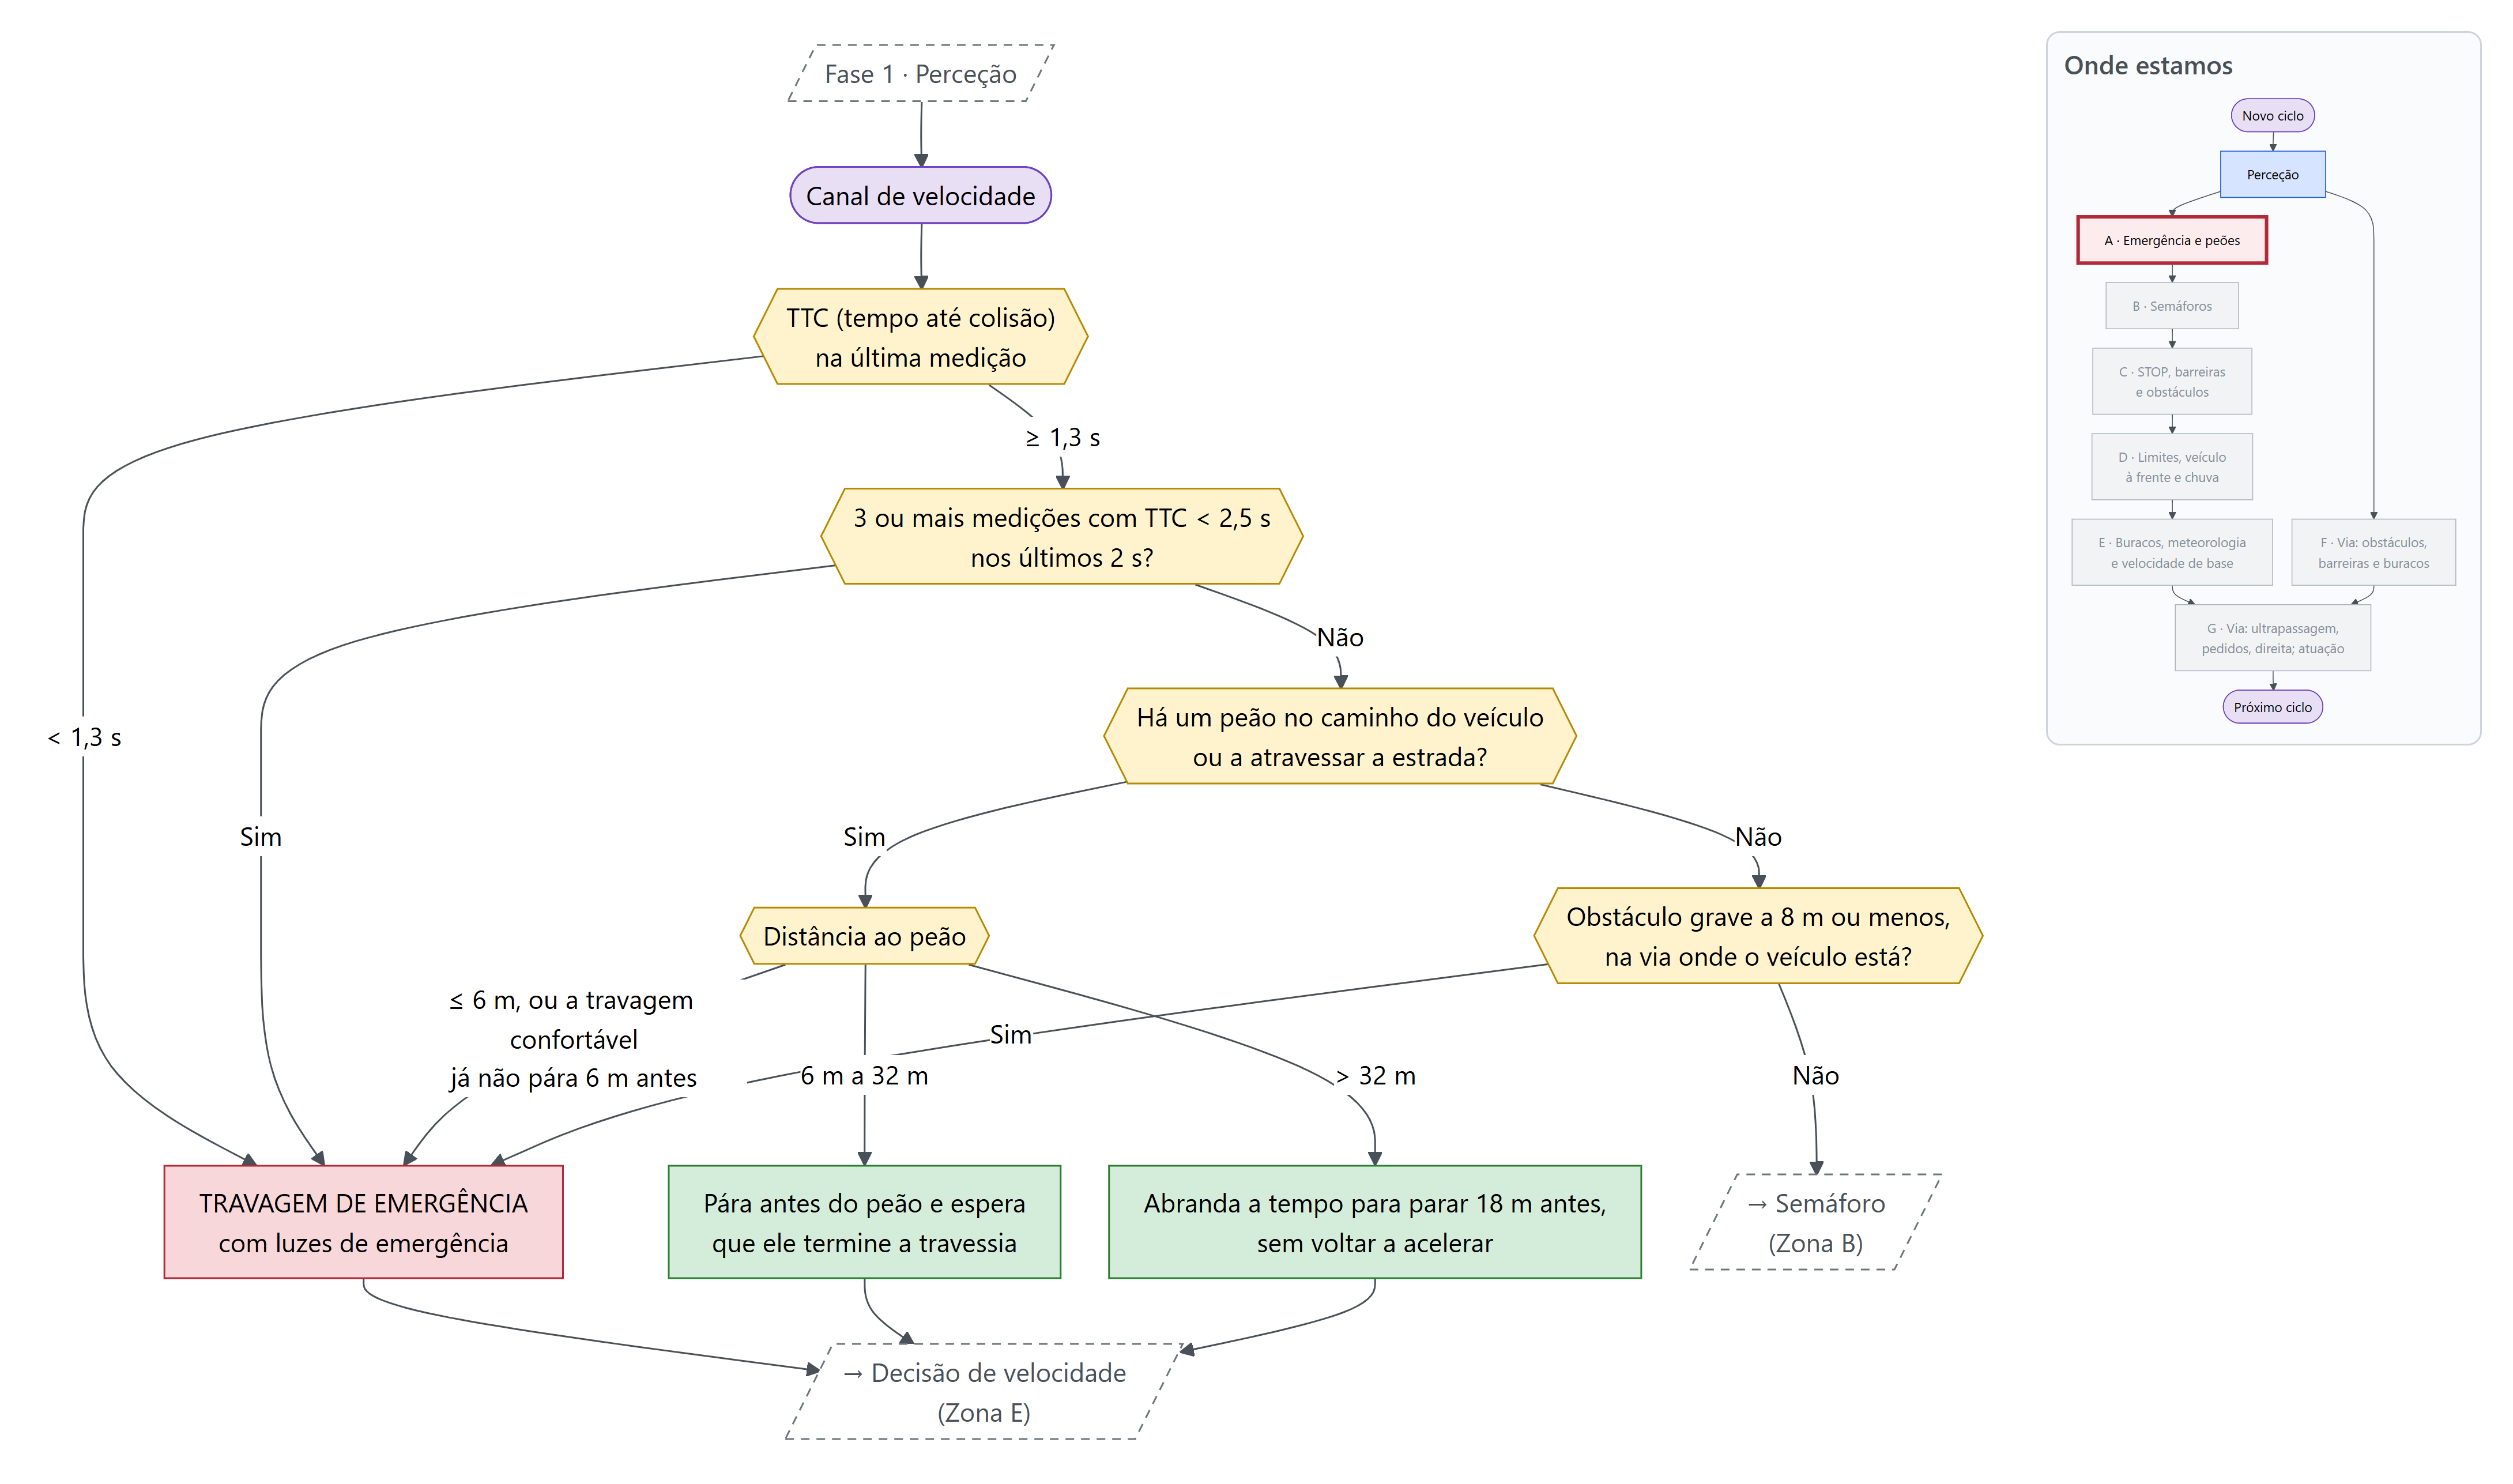
\includegraphics[width=\linewidth,height=0.80\textheight,keepaspectratio]{figuras/fig12_zona_a_emergencia_e_peoes}
\caption{Zona A: emergência e peões}\label{fig:12}
\end{figure}

\begin{landscape}
\begin{figure}[H]
\centering
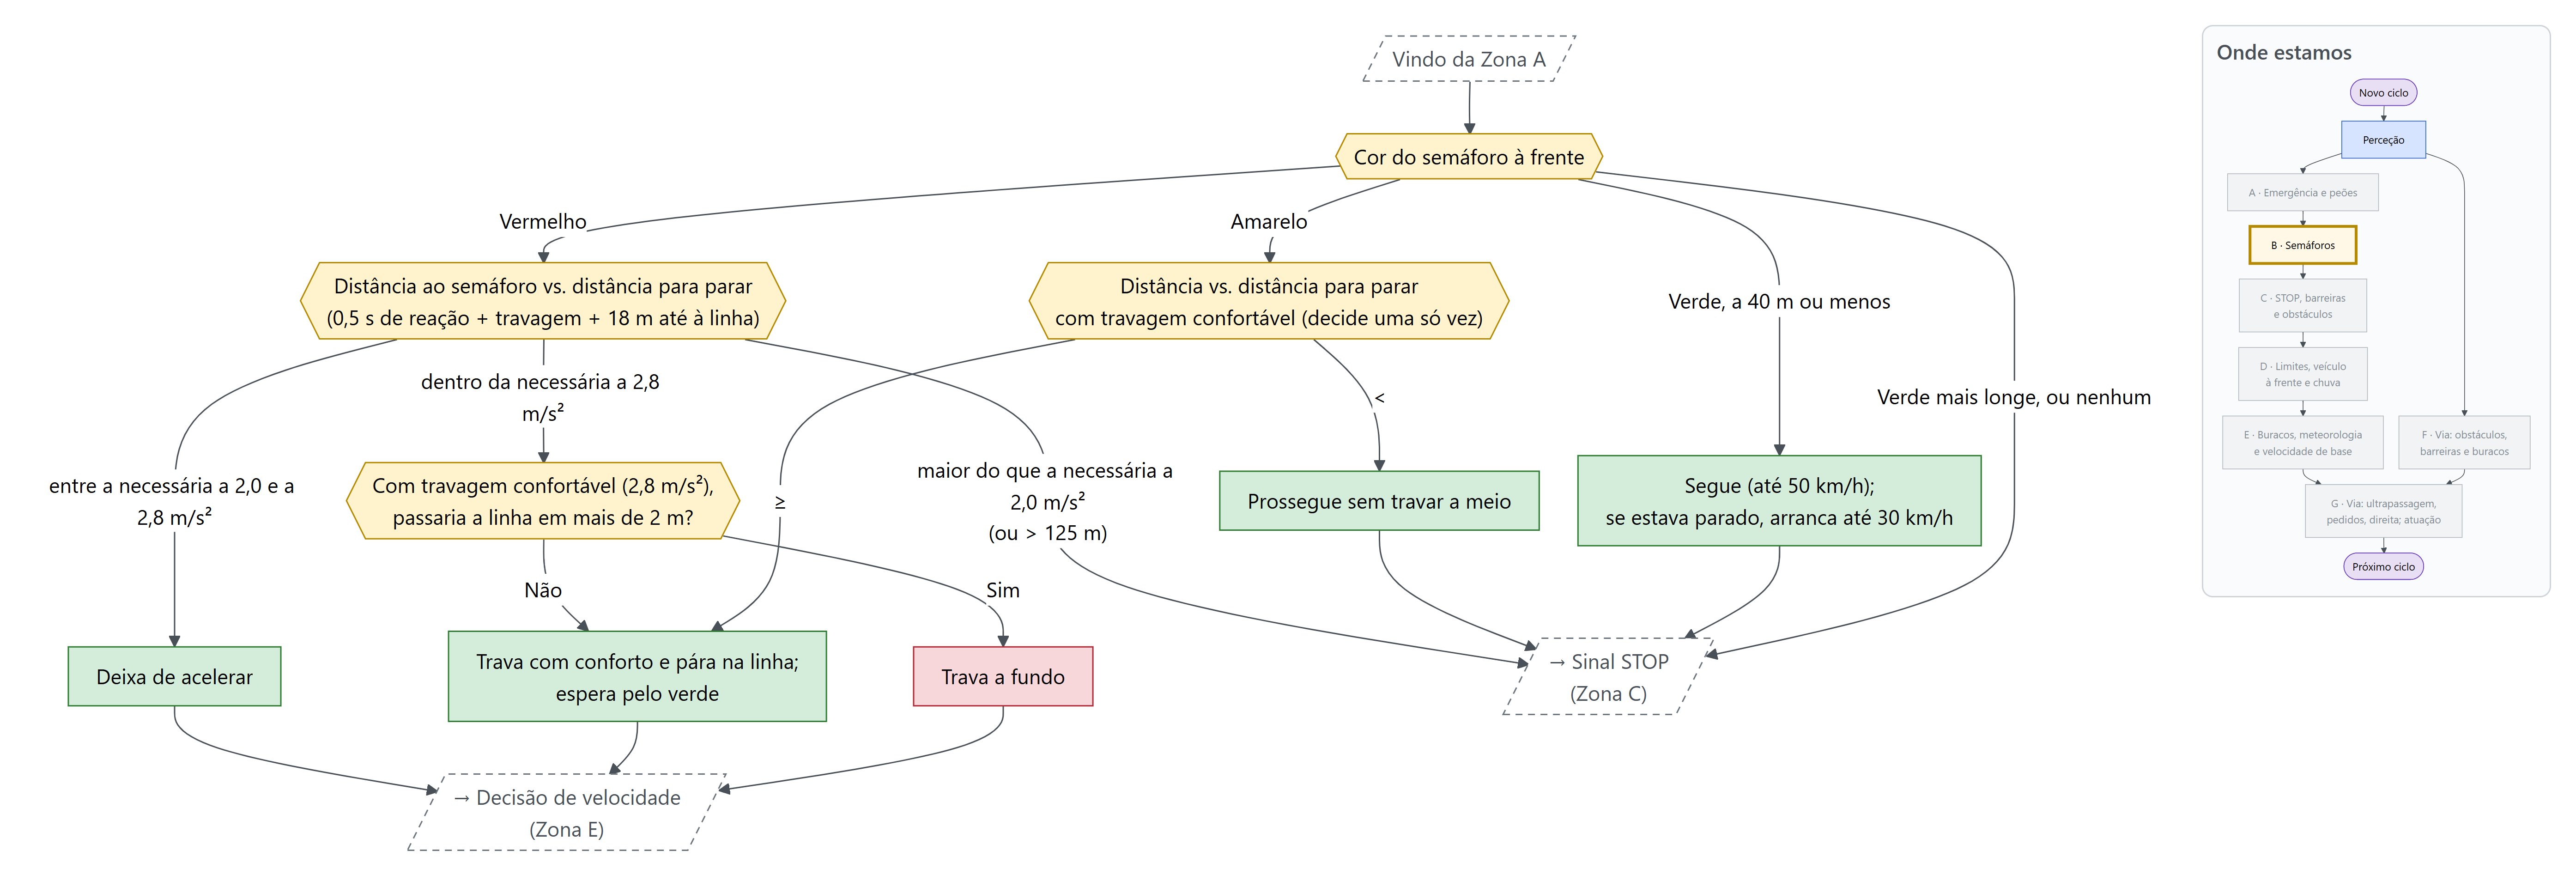
\includegraphics[width=\linewidth,height=0.82\textheight,keepaspectratio]{figuras/fig13_zona_b_semaforos}
\caption{Zona B: semáforos}\label{fig:13}
\end{figure}
\end{landscape}

\begin{landscape}
\begin{figure}[H]
\centering
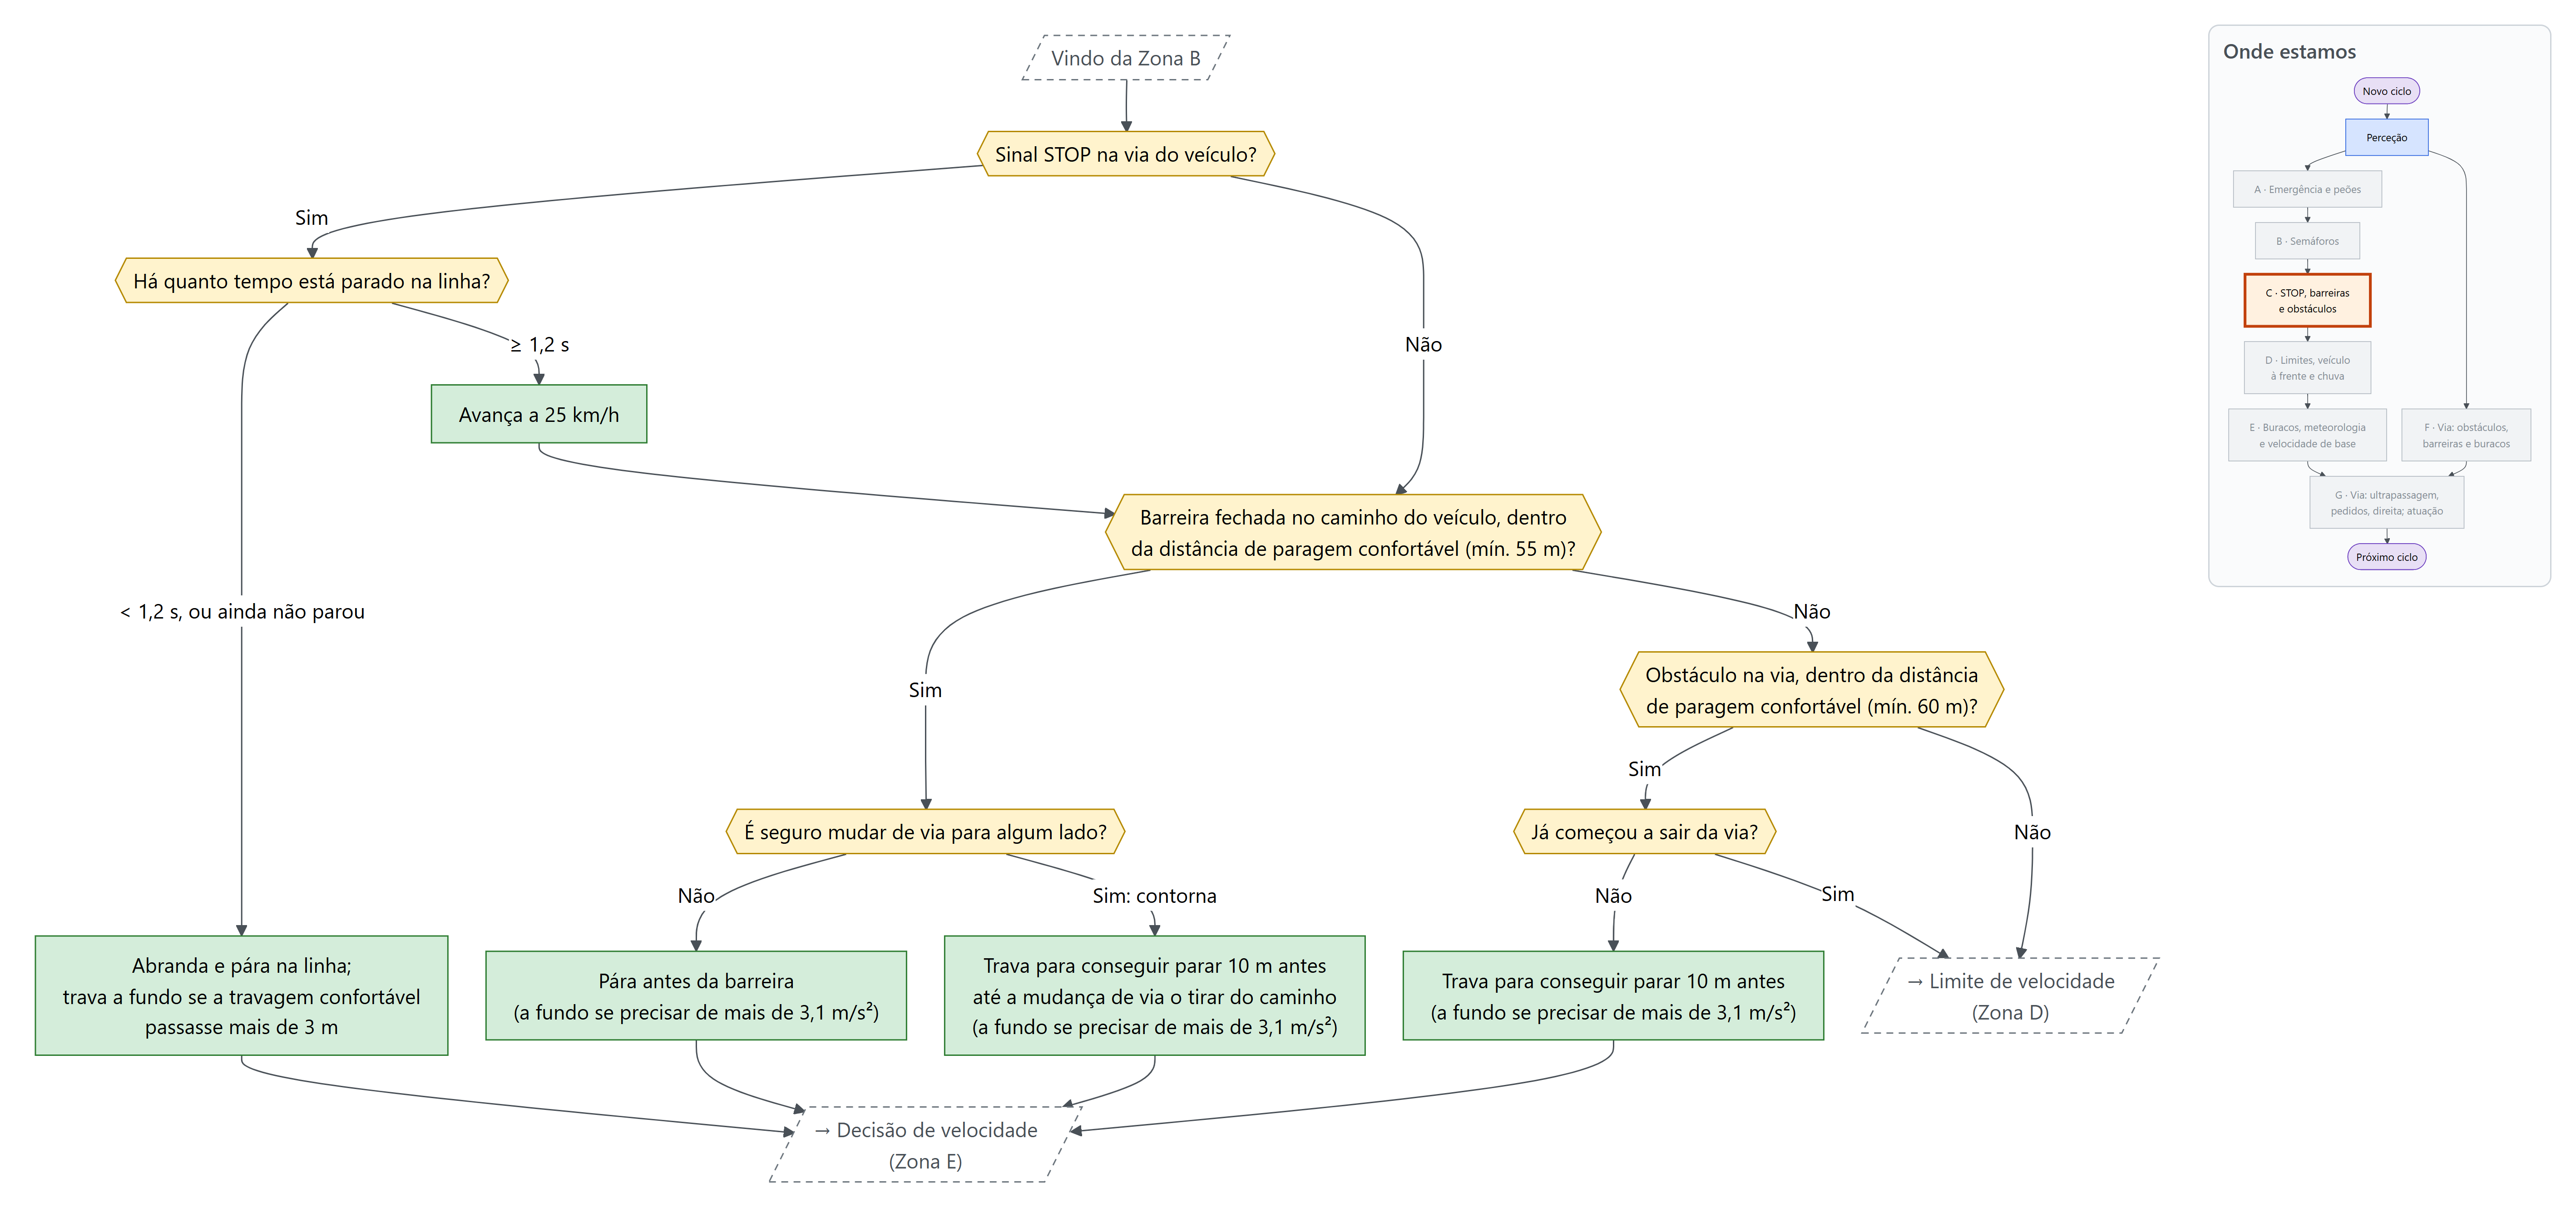
\includegraphics[width=\linewidth,height=0.82\textheight,keepaspectratio]{figuras/fig14_zona_c_stop_barreiras_e}
\caption{Zona C: STOP, barreiras e obstáculos}\label{fig:14}
\end{figure}
\end{landscape}

\begin{figure}[H]
\centering
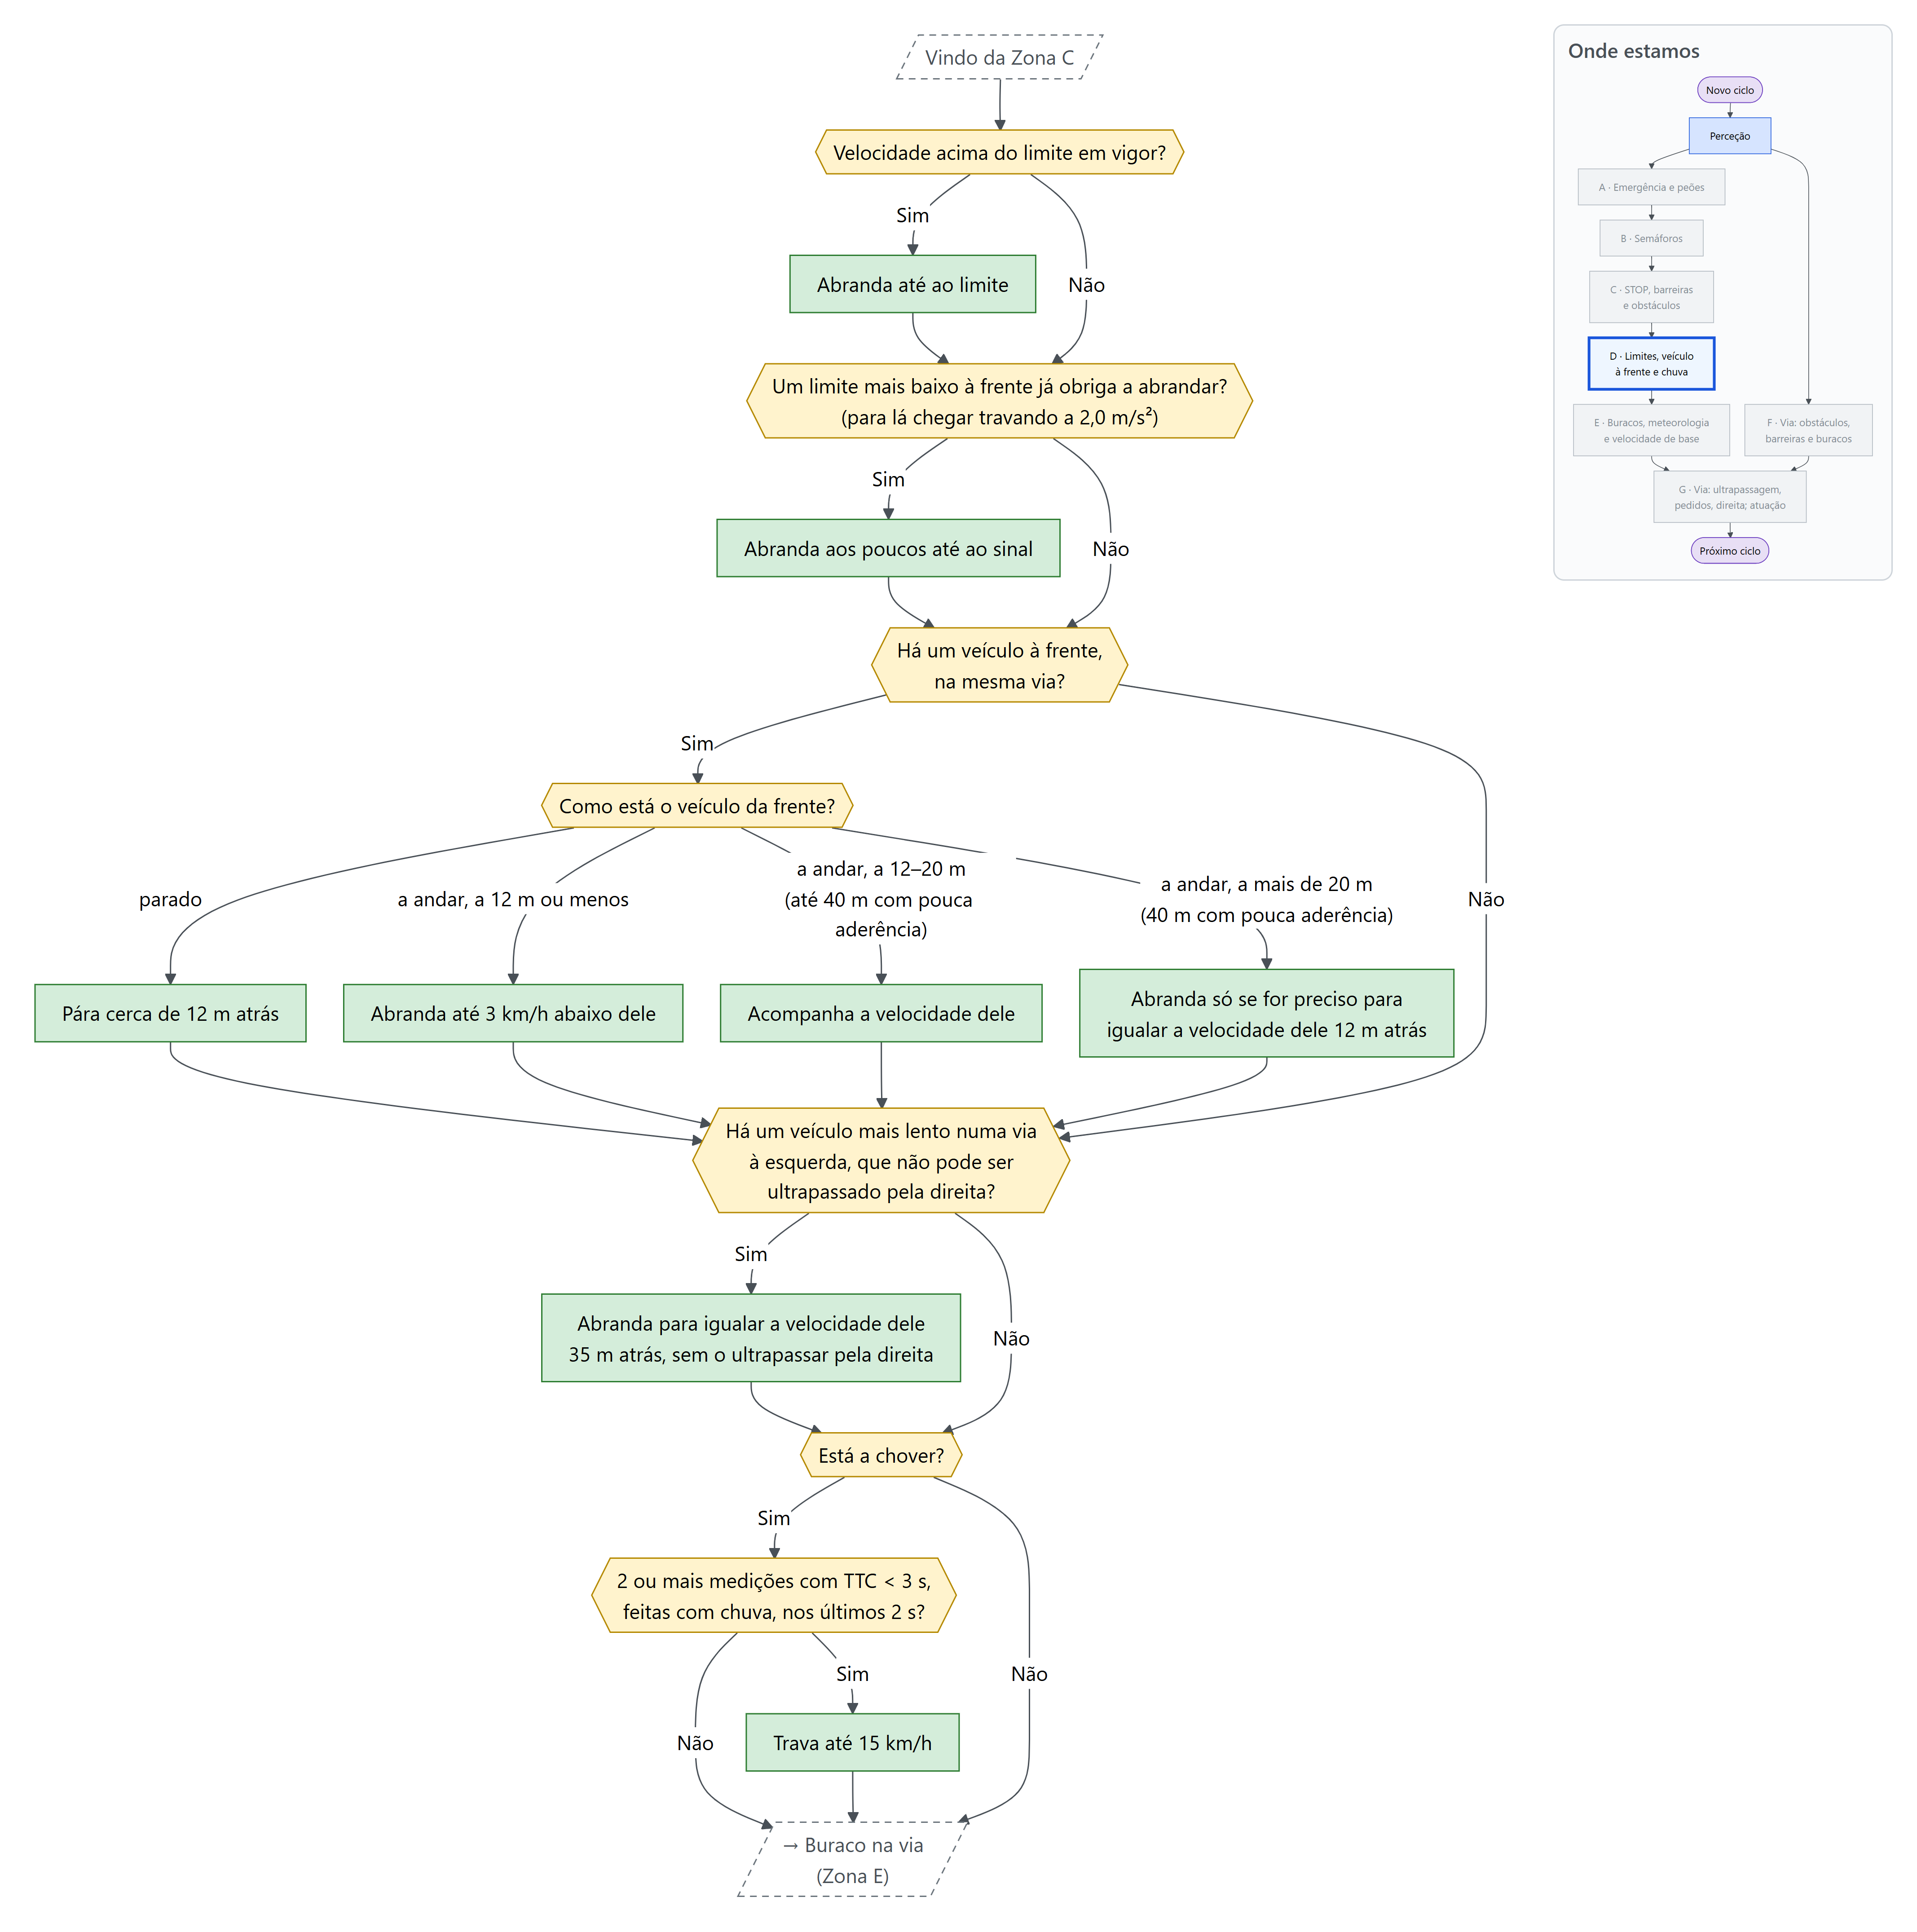
\includegraphics[width=\linewidth,height=0.80\textheight,keepaspectratio]{figuras/fig15_zona_d_limites_veiculo_a_frente}
\caption{Zona D: limites, veículo à frente e chuva}\label{fig:15}
\end{figure}

\begin{figure}[H]
\centering
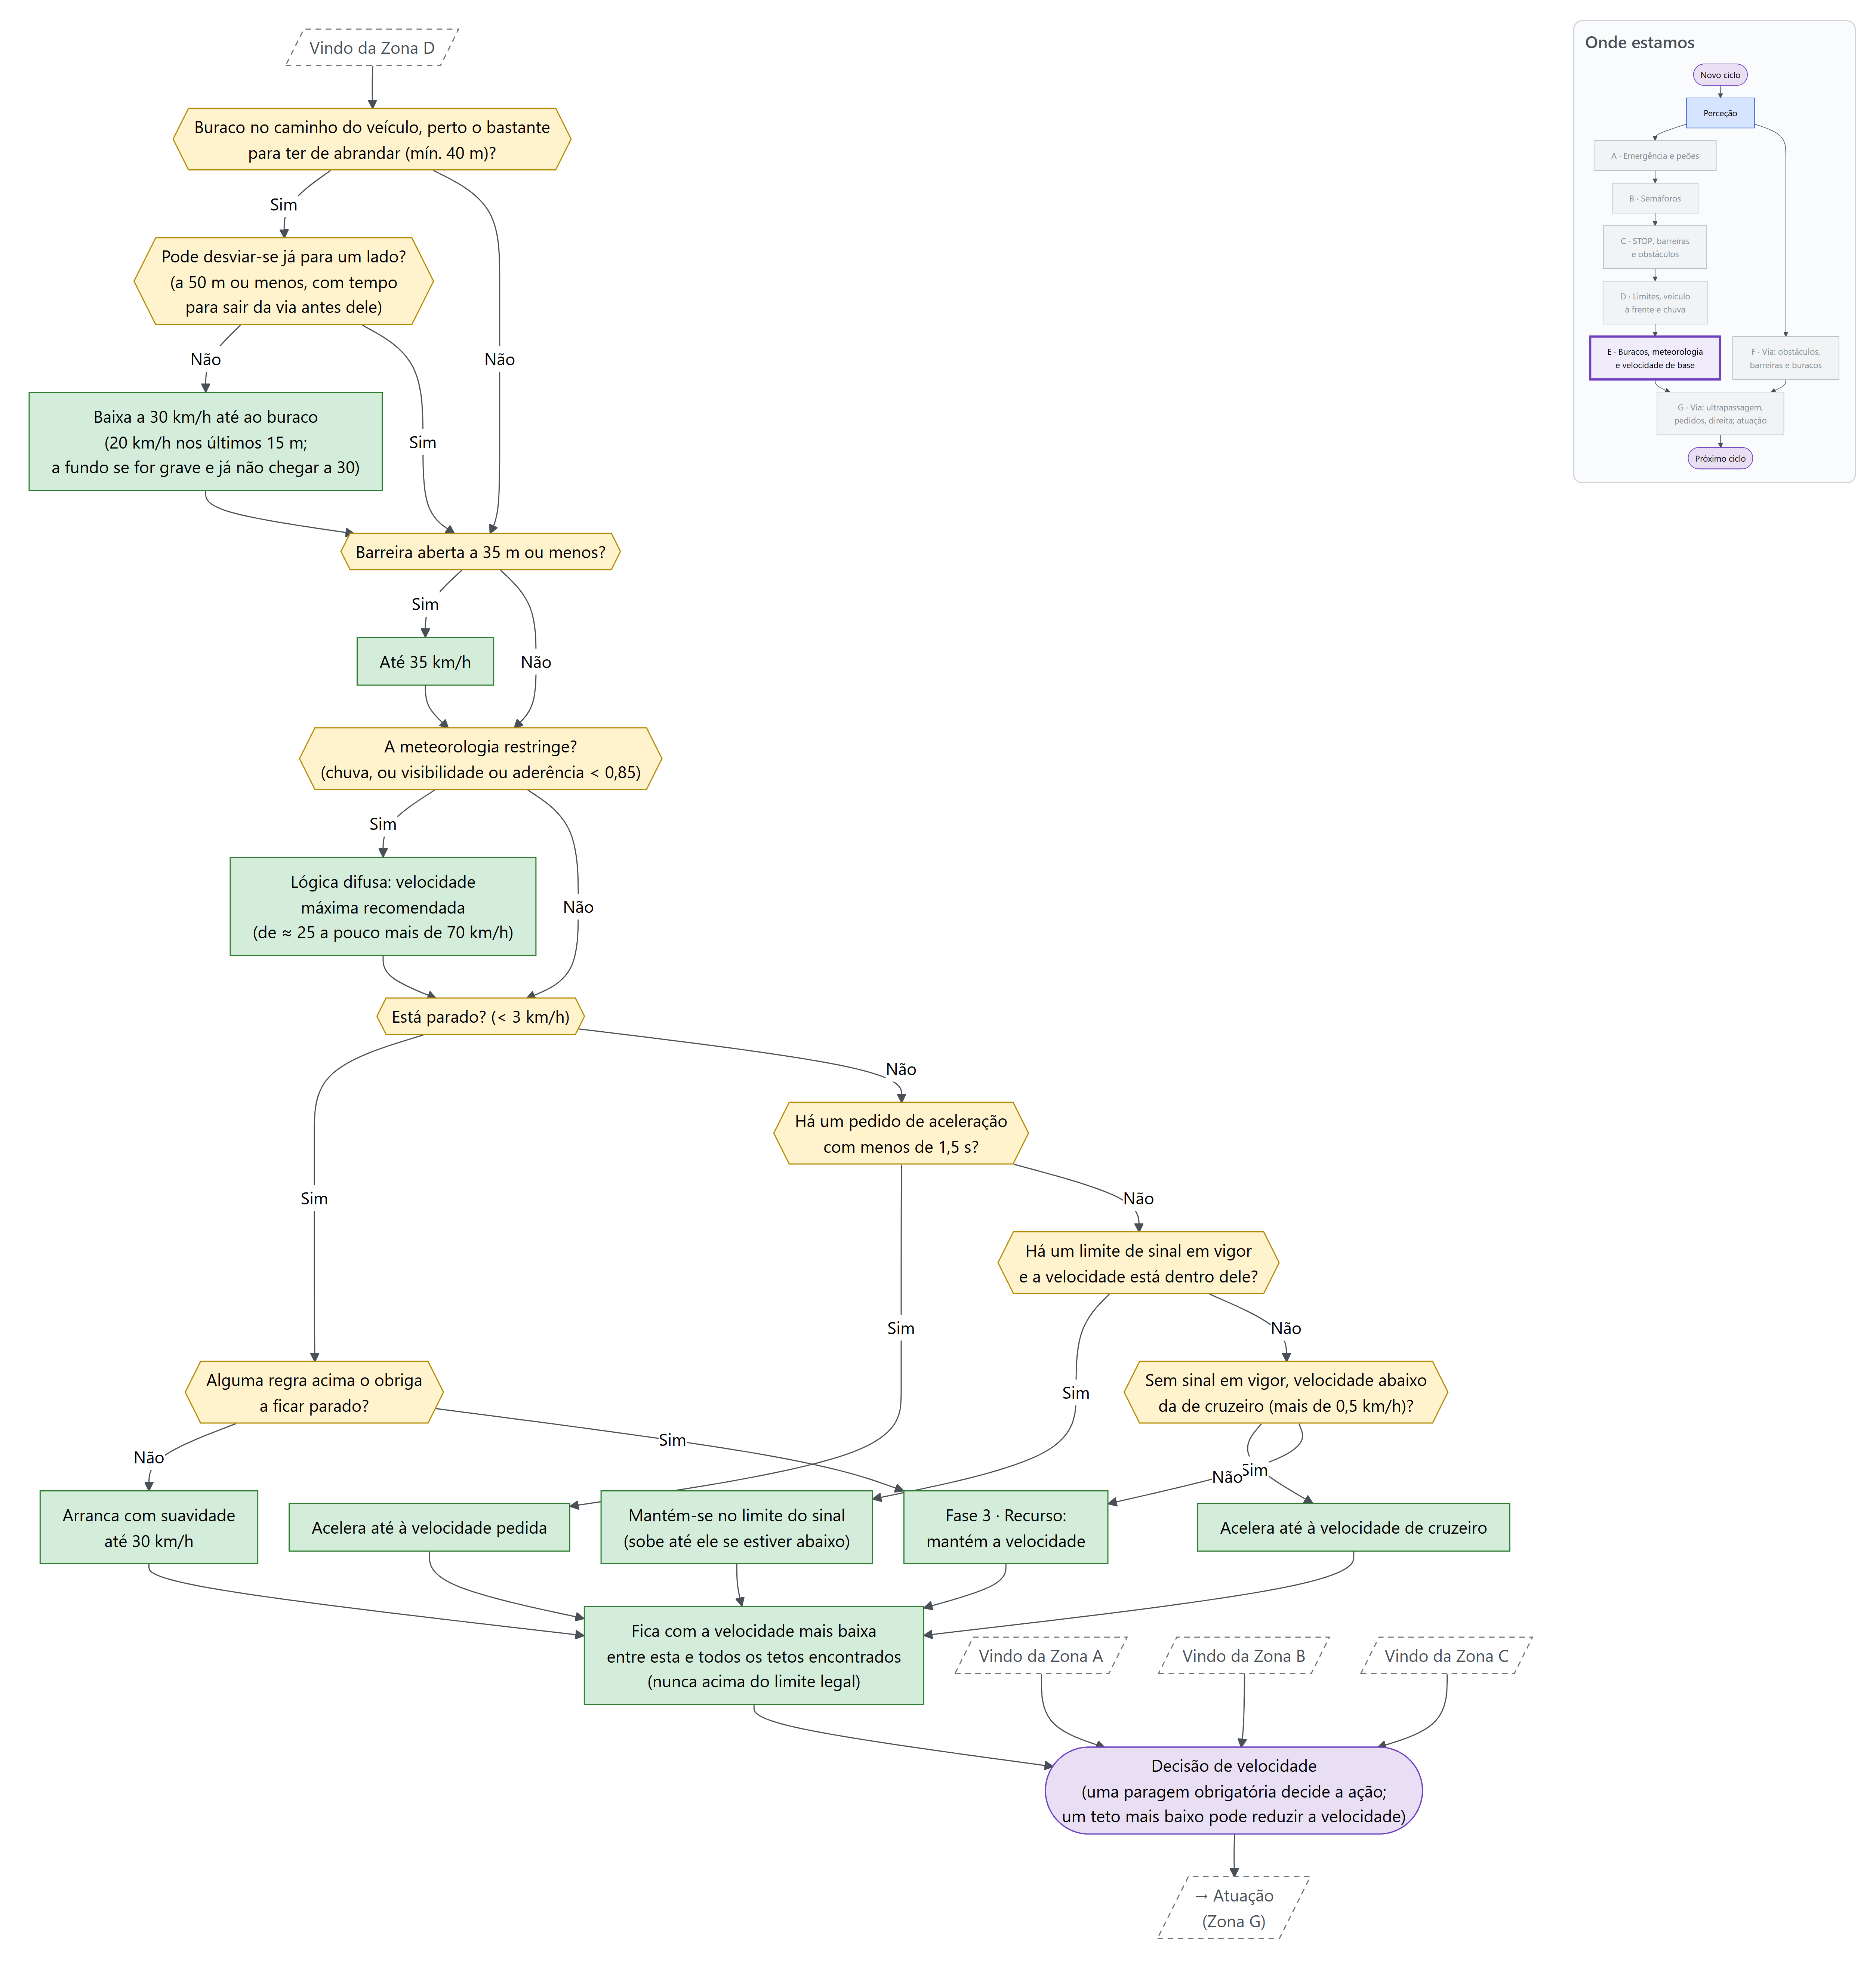
\includegraphics[width=\linewidth,height=0.80\textheight,keepaspectratio]{figuras/fig16_zona_e_buracos_meteorologia_e}
\caption{Zona E: buracos, meteorologia e velocidade de base}\label{fig:16}
\end{figure}

\begin{landscape}
\begin{figure}[H]
\centering
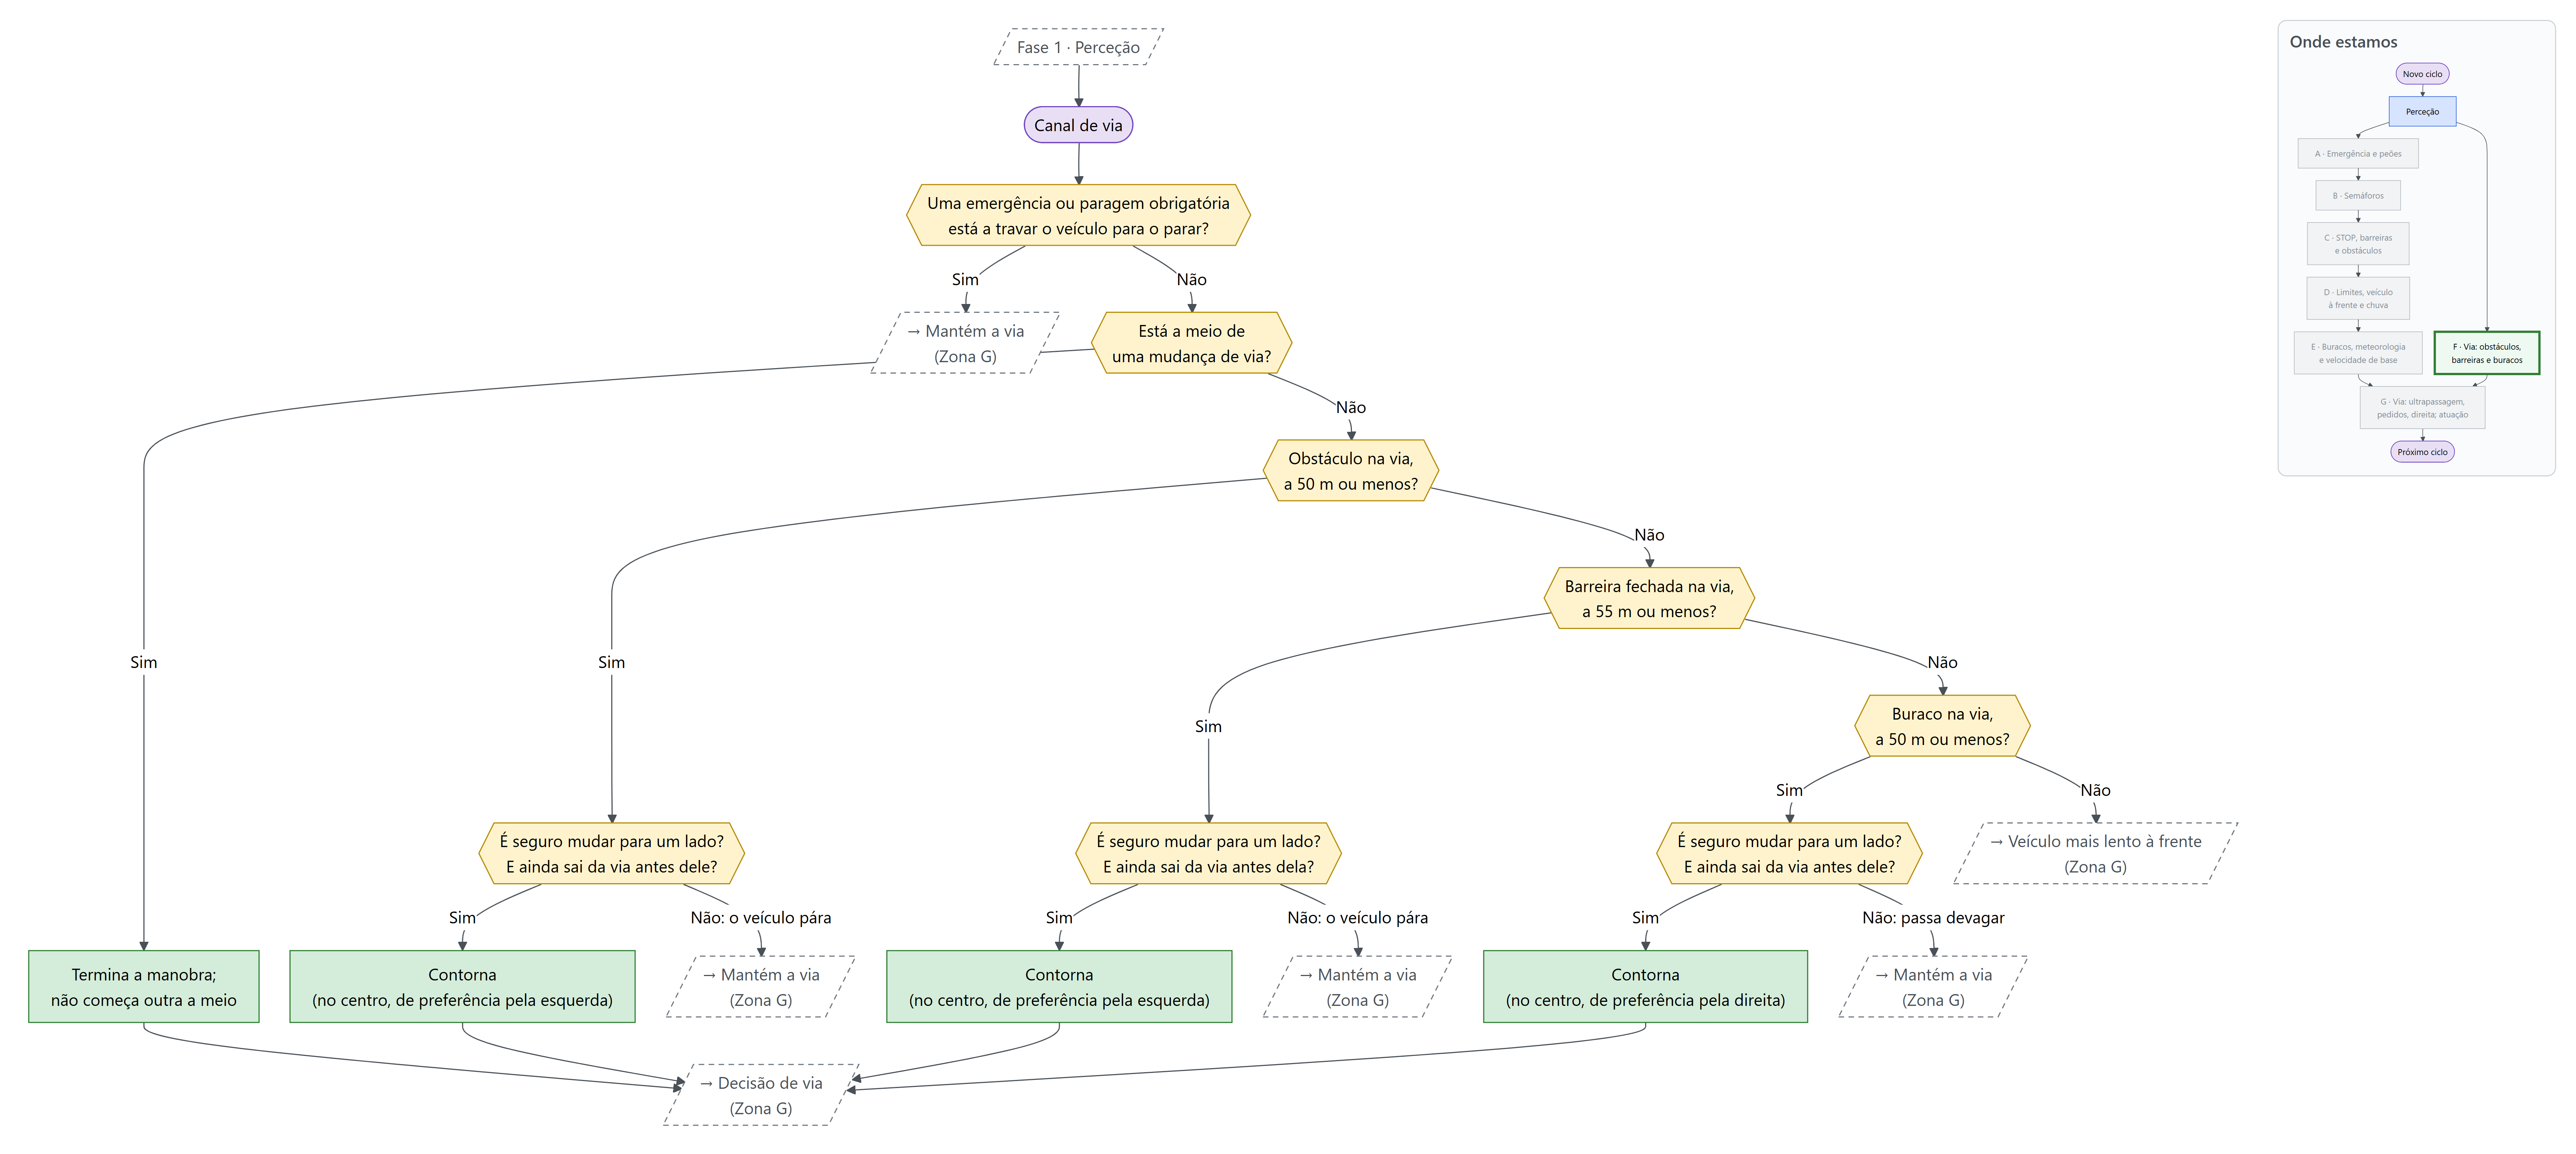
\includegraphics[width=\linewidth,height=0.82\textheight,keepaspectratio]{figuras/fig17_zona_f_canal_de_via_perante}
\caption{Zona F: canal de via perante obstáculos, barreiras e buracos}\label{fig:17}
\end{figure}
\end{landscape}

\begin{figure}[H]
\centering
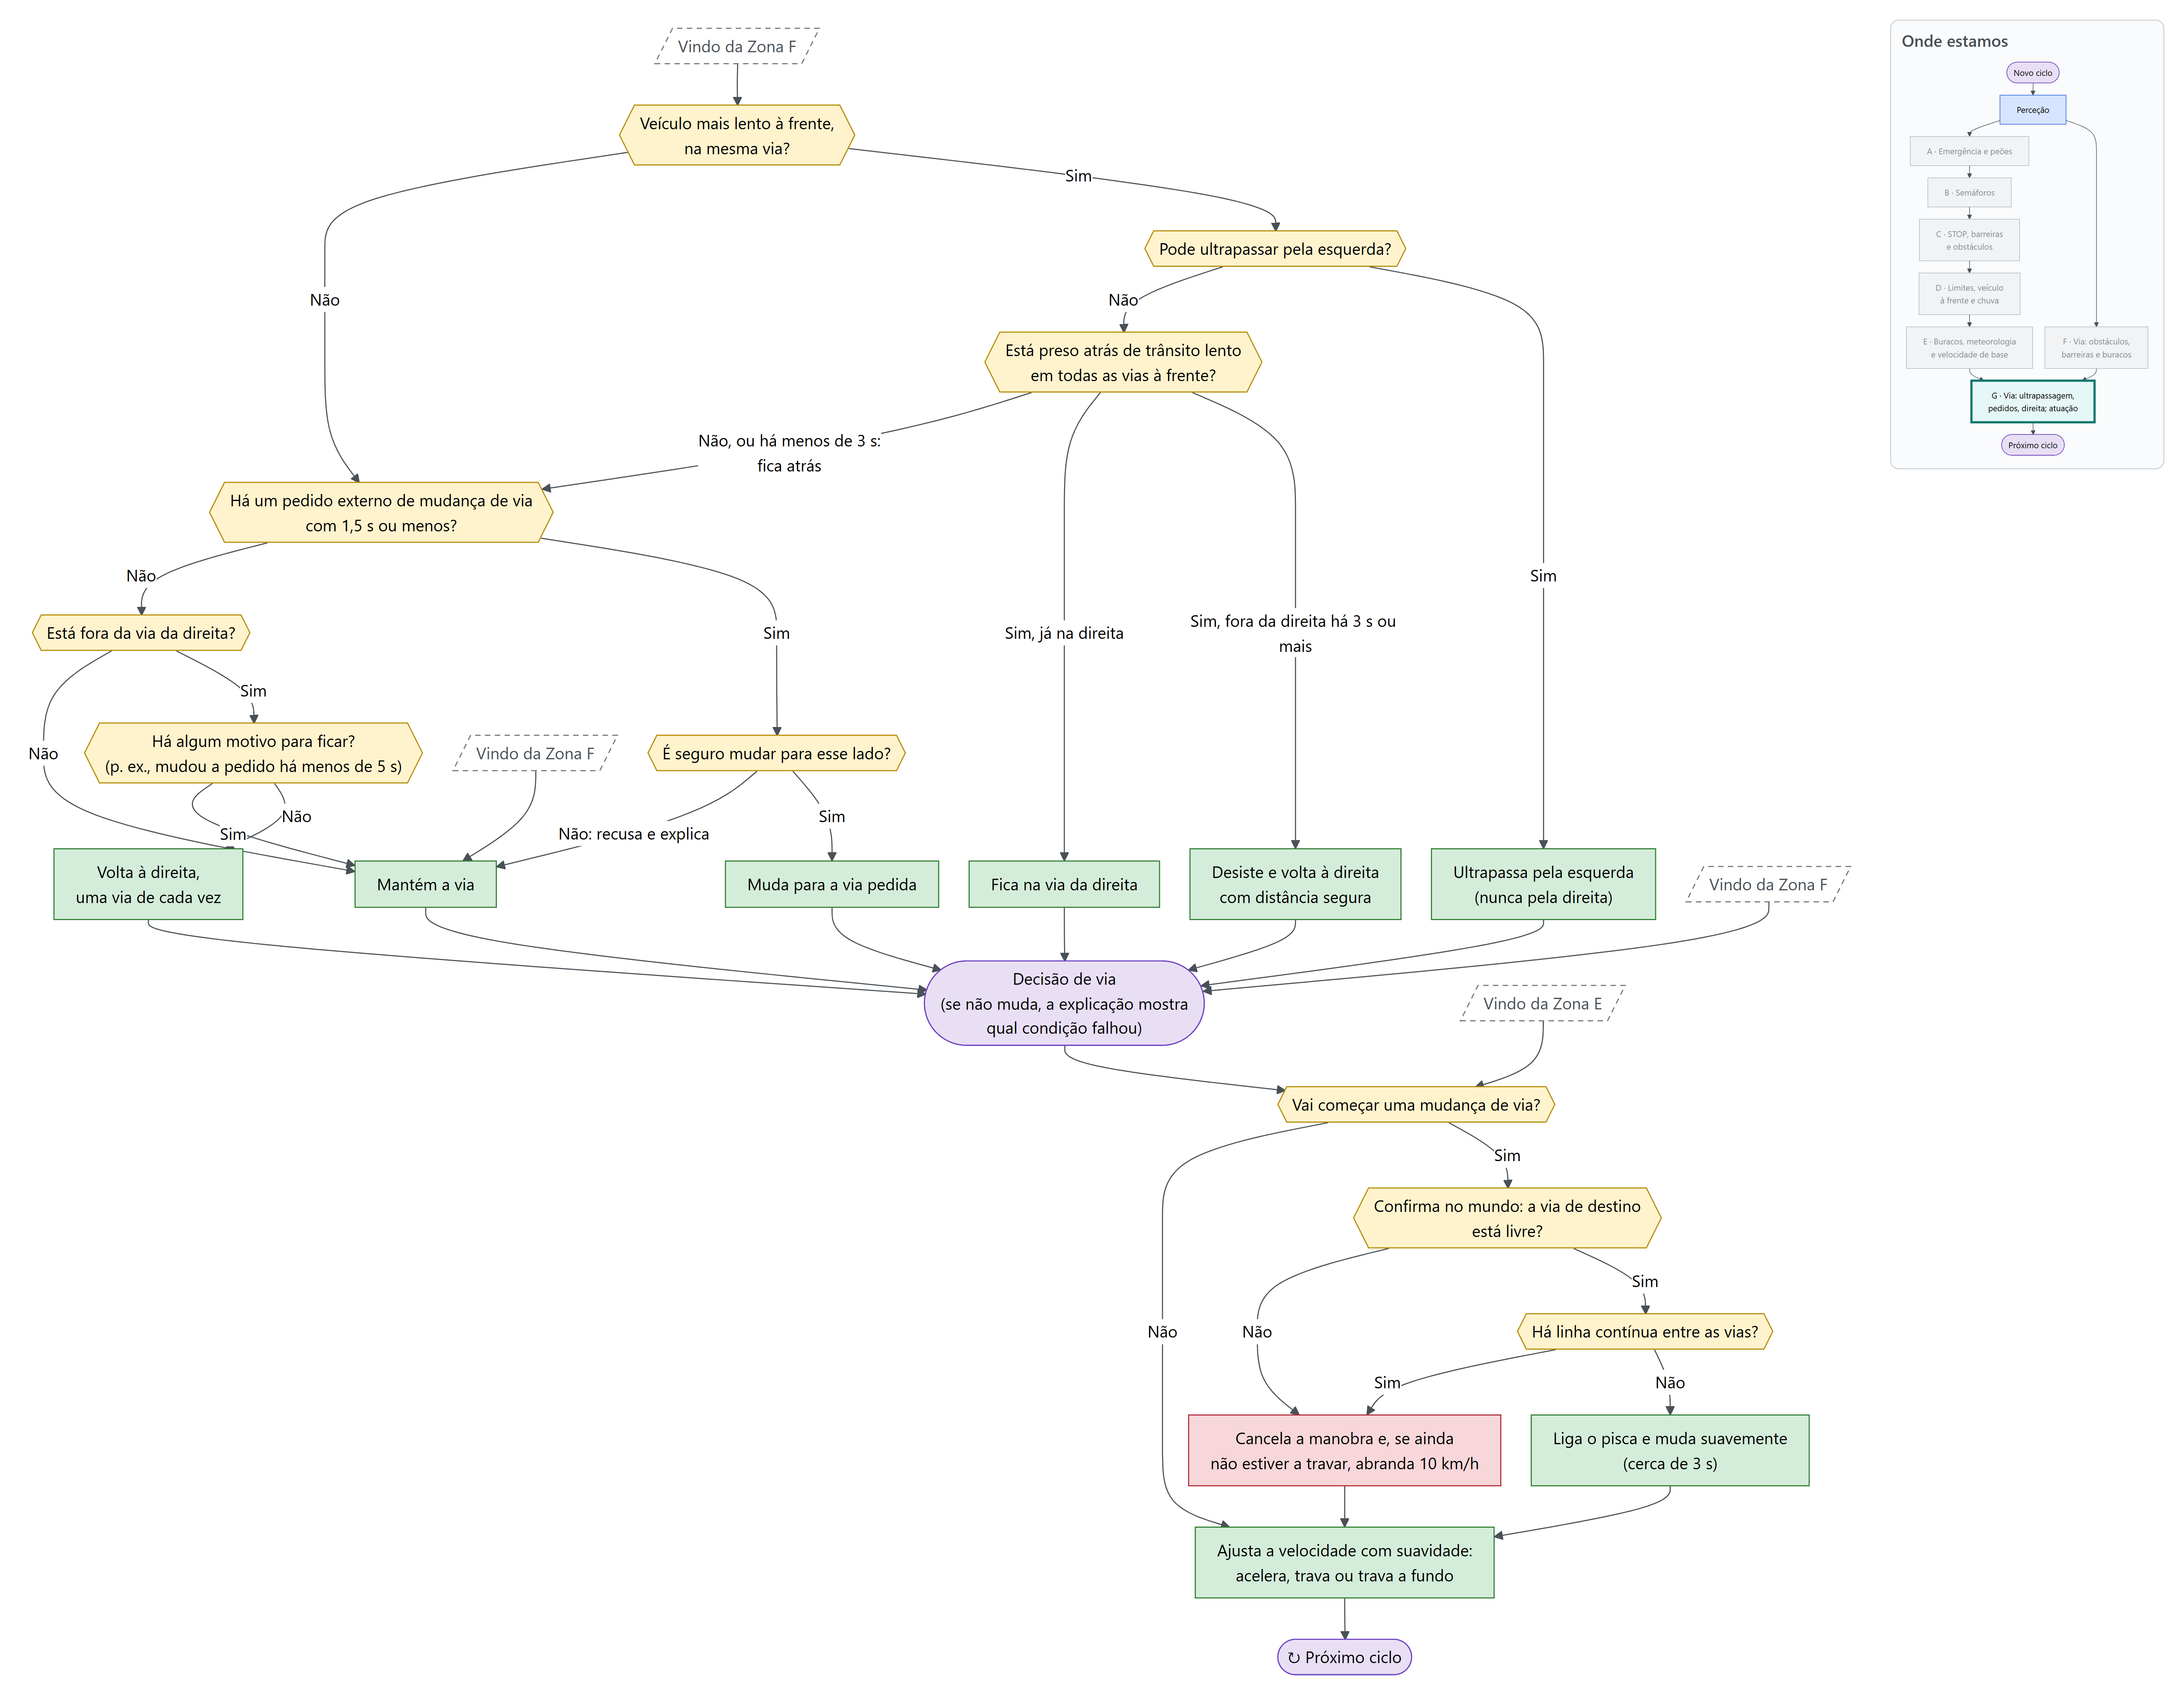
\includegraphics[width=0.90\linewidth,height=0.80\textheight,keepaspectratio]{figuras/fig18_zona_g_ultrapassagem_pedidos}
\caption{Zona G: ultrapassagem, pedidos, regresso à direita e atuação}\label{fig:18}
\end{figure}


\end{document}
